\documentclass[11pt,aspectratio=169]{beamer}

% --- Tema og fonte ---
\usetheme{Madrid}
\usefonttheme{serif}
% --- Farver ---
\definecolor{myteal}{RGB}{14,71,57}
\setbeamercolor{title}{fg=white}
\setbeamercolor{frametitle}{fg=white,bg=myteal}
\setbeamercolor{block title}{fg=white,bg=myteal}
\setbeamercolor{block body}{bg=myteal!10}
\setbeamercolor{normal text}{fg=myteal}
\setbeamercolor{background canvas}{bg=white}
\setbeamercolor{structure}{fg=myteal}
\setbeamercolor{palette primary}{fg=white,bg=myteal}
\setbeamercolor{palette secondary}{fg=white,bg=myteal!80}
\setbeamercolor{palette tertiary}{fg=white,bg=myteal!60}
\setbeamercolor{author in head/foot}{fg=white,bg=myteal}
\setbeamercolor{title in head/foot}{fg=white,bg=myteal!80}
\setbeamercolor{date in head/foot}{fg=white,bg=myteal!60}
\setbeamercolor{titlelike}{fg=myteal}
\setbeamercolor{section in toc}{fg=myteal}
\setbeamercolor{item}{fg=myteal}
% --- Sprog og encoding ---
\usepackage[utf8]{inputenc}
\usepackage[danish]{babel}
\usepackage[T1]{fontenc}
\usepackage{lmodern}
% --- Matematik ---
\usepackage{amsmath,amsfonts,amssymb}
% --- Grafik og layout ---
\usepackage{graphicx}
\usepackage{ragged2e}
\usepackage{booktabs}
\usepackage{arydshln}
\usepackage[most]{tcolorbox}
% --- Ikoner og figurer ---
\usepackage{fontawesome5}
\usepackage{tikz}
\usetikzlibrary{positioning,arrows.meta,shapes.geometric,calc}
\usepackage{circuitikz}
% --- Positionering ---
\usepackage[absolute,overlay]{textpos}
% --- CSV ---
\usepackage{csvsimple}
% --- Kildehenvisning nederst på slides ---
\setbeamercolor{framesource}{fg=gray,bg=white}
\setbeamerfont{framesource}{size=\scriptsize}
\newcommand{\framesource}[1]{%
  \begin{textblock*}{12cm}(0.5cm,8.6cm)
    \raggedleft
    \beamercolorbox[wd=\textwidth,rightskip=0.5cm]{framesource}{#1}
  \end{textblock*}
}
% --- Automatisk billedattribution ---
\csvreader[
  head to column names,
  no head
]{Billeder/billedkilder.csv}{}{}
\newcommand{\billedkilde}[1]{%
  \csvreader[
    head to column names,
    full filter=\ifcsvstrcmp{\filnavn}{#1}{\csvfilteraccept}{\csvfilterreject},
    no head
  ]{Billeder/billedkilder.csv}{}%
  {%
    \tiny\forfatter\ / Wikimedia Commons (\licens)%
  }%
}
% --- Boksstile til jagttid-sliden ---
\tcbset{
  gruppe/.style={
    enhanced,
    colback=white,
    colframe=myteal,
    coltitle=myteal,
    boxrule=0.8pt,
    dashed,
    sharp corners,
    fonttitle=\bfseries\large,
    attach boxed title to top left={yshift=-2mm,xshift=3mm},
    boxed title style={colback=white,colframe=white,boxrule=0pt,sharp corners},
    top=1mm,left=1mm,right=1mm,bottom=1mm
  },
  felt/.style={
    enhanced,
    colback=white,
    colframe=myteal,
    boxrule=0.6pt,
    sharp corners,
    halign=center,
    valign=center,
    width=\linewidth,
    height=1.55cm,
    fit,
    fit algorithm=fontsize,
    fit basedim=7pt,
    boxsep=0.3mm,
    left=0.5mm, right=0.5mm, top=0.3mm, bottom=0.3mm
  },
  feltfri/.style={
    enhanced,
    colback=white,
    colframe=myteal,
    boxrule=0.6pt,
    sharp corners,
    halign=center,
    valign=center,
    width=\linewidth,
    boxsep=0.3mm,
    left=0.5mm, right=0.5mm, top=0.3mm, bottom=0.3mm,
    fontupper=\scriptsize
  }
}
% --- Matematiske operatorer ---
\DeclareMathOperator{\sen}{sen}
\DeclareMathOperator{\tg}{tg}
% --- Beamer-indstillinger ---
\setbeamertemplate{caption}[numbered]
\setbeamertemplate{navigation symbols}{}
% --- Forfatter ---
\author[Østerbro Jagttegn]{Østerbro Jagttegn \\ \textbf{Aleksander Sønder}}
% --- Hyperref (altid sidst) ---
\usepackage{hyperref}
\hypersetup{
  colorlinks=true,
  linkcolor=myteal,
  urlcolor=myteal,
  citecolor=myteal
}

\title{Obligatorisk Teori 5}
\date{\today}

\begin{document}

% Titelside
\begin{frame}
  \titlepage
\end{frame}

% Indholdsfortegnelse (valgfri)
\begin{frame}{Program}
  \tableofcontents
\end{frame}

\section{Jagtetiske regler for kronvildt}

\begin{frame}
  \vspace{3em}
  \begin{center}
    {\LARGE \textbf{Jagtetiske regler for kronvildt}
    }
    \\
    \vspace{1em}
    Vildtforvaltningsrådet \\
    https://sgavmst.dk/media/vcupseet/de-jagtetiske-regler-for-kronvildt.pdf
  \end{center}
\end{frame}

\begin{frame}{Formål \& Ansvar}
\begin{itemize}
\item Sikre bred offentlig accept af kronvildtjagt – grundlag for fortsat jagt uden stramme restriktioner
\item Regler udarbejdet af Vildtforvaltningsrådet
\item Den enkelte jægers ansvar: Værne om kronvildt og jagten ved at følge reglerne
\item Fokus: Naturlig bestand, nabohensyn, bæredygtighed, ren skydning og minimal forstyrrelse
\end{itemize}
\end{frame}

\begin{frame}{Afskydningspolitik}
\begin{itemize}
\item Tilrettelæg afskydning for naturlig køns- og aldersfordeling
\item Størst afskydning blandt unge dyr (kalve + unghjorte/unghinder)
\item Jævn fordeling mellem handyr og hundyr
\item Indskrænk septemberjagten på hjorte mest muligt → giver ro i brunsten
\item Undgå ubalance (mange hjorte – få hinder/kalve)
\end{itemize}
\end{frame}

\begin{frame}{Nabohensyn \& Terrænstørrelse}
\begin{itemize}
\item Afskydning skal stå i rimeligt forhold til terrænets størrelse
\item Sigt mod at vildt falder på eget område (kronvildt går ofte 100 m+)
\item Ikke flere end 1 stk. pr. sæson på arealer mindre end 25 ha
\item På små/smalle arealer: Indgå naboaftaler eller fælles jagt/forståelse
\item Skel mellem kerneområder (sædvanlig ophold) og vandringsområder
\end{itemize}
\end{frame}

\begin{frame}{Bæredygtig jagtudnyttelse}
\begin{itemize}
\item Bæredygtighed vurderes lokalt – ikke nationalt
\item Typisk max 1 stk. pr. 25–50 ha pr. sæson (lavere på større ejendomme)
\item Kerneområder (ro, dækning, føde) tåler højere afskydning pr. ha
\item Yderområder: Lavere afskydning for at etablere fast bestand
\item Kronvildt har store revirer → elastisk bæredygtighedsbegreb
\end{itemize}
\end{frame}

\begin{frame}{Skydning \& Skydefærdigheder}
\begin{itemize}
\item Vær sikker på, hvad du skyder på – hold hovedet koldt ved dyr i rudel
\item Foretræk sideskud – skyd helst på dyr i ro
\item Ingen chancebetonede skud – træn på skive + bevægeligt mål
\item Kend dine begrænsninger – træn også luftbøsse/bevægelige mål/tørtræning
\item Brug hochsitz/hochstand når muligt
\end{itemize}
\end{frame}

\begin{frame}{Anskydninger \& Eftersøgning}
\begin{itemize}
\item Vær meget opmærksom på skudtegn
\item Skyd ikke til friskt dyr, hvis tidligere skudt dyr ikke ligger synligt forendt
\item Brug altid schweisshund ved tvivl/anskydning
\item Afmærk præcist ved tvivl – tilkald erfaren schweisshundefører
\item Hjælp hundefører med gode observationer – undgå flere skud i samme område
\item Mål: Minimal antal anskydninger – skylder vi kronvildtet og hinanden
\end{itemize}
\end{frame}

\begin{frame}{Jagtudøvelse \& Forstyrrelser}
\begin{itemize}
\item Ingen tryk-/drivjagter i september (brunsten)
\item Skyd ikke diegivende hinder i oktober (kalve dier stadig)
\item Min. 3 uger mellem tryk-/drivjagter
\item Max 3–4 fællesjagter pr. sæson på samme revir
\item Begræns hurtigtgående store hunde til drivjagt
\item Pürsch foretrækkes – undgå simultan pürsch over hele terræn
\item Frihold områder under fællesjagter – kronvildt kræver ro (især i etableringsfase)
\end{itemize}
\end{frame}

\begin{frame}{Dialog \& Regionale Krondyrgrupper}
\begin{itemize}
\item Planlæg afskydning lokalt sammen med naboer/lodsejere
\item Indgå i (formelle/uformelle) samarbejder om bestand og skader
\item Bidrag til fælles ansvarsfølelse
\item Regionale Krondyrgrupper understøtter efterlevelse af reglerne
\item Bred repræsentation → bedre dialog og forvaltning
\end{itemize}

\bigskip
\textbf{Sammenfatning: Kronvildtjagt kræver særligt hensyn – forvaltes med respekt, samarbejde og selvbegrænsning.}
\end{frame}

\section{Våben og ammunition til jagt}

\begin{frame}
  \vspace{3em}
  \begin{center}
    {\LARGE \textbf{Bekendtgørelse om våben og ammunition der må anvendes til jagt m.v.}} \\
    \vspace{1em}
    BEK nr 1479 af 05/12/2023 \\ §§ 1-3
  \end{center}
\end{frame}

\begin{frame}{Tilladte skydevåben til jagt og regulering (§1)}
    \begin{itemize}
        \item \textbf{Glatløbede haglgeværer}:
          \begin{itemize}
            \item Pibelængde ≥ 55 cm
            \item Højst kaliber 12
            \item Højst 2 patroner (permanent begrænsning hvis konstrueret til mere)
          \end{itemize}
        \item \textbf{Riflede våben}:
          \begin{itemize}
            \item Manuelt repeterende
            \item Ikke helautomatiske/fuldautomatiske
            \item Halvautomatiske: Højst 3 patroner (permanent begrænsning hvis mere; max 2 i magasin + 1 i kammer)
            \item Luftgeværer: Min projektildiameter ≥ 5,5 mm
          \end{itemize}
        \item \textbf{Forbudt}: Revolvere og pistoler
    \end{itemize}
\end{frame}

\begin{frame}{Jagtammunition til riflede våben}
\framesubtitle{Tilladt ammunition til jagt og regulering af vildt}

\tiny
\begin{tabular}{|c|p{2.8cm}|c|c|c|c|c|}
\hline
\textbf{Klasse} & \textbf{Vildtart} &
\textbf{\begin{tabular}{@{}c@{}}Kuglediam.\\$\geq$6 mm\\$E_{100}\geq$2000 J\end{tabular}} &
\textbf{\begin{tabular}{@{}c@{}}Kuglediam.\\$\geq$5,5 mm\\$E_{100}\geq$800 J\end{tabular}} &
\textbf{\begin{tabular}{@{}c@{}}$E_{100}$\\$\geq$175 J\end{tabular}} &
\textbf{\begin{tabular}{@{}c@{}}$E_0$\\$\geq$150 J\end{tabular}} &
\textbf{\begin{tabular}{@{}c@{}}$V_0$\\$\geq$200\\m/sek.\textsuperscript{*}\end{tabular}} \\
\hline
1 & Kronvildt, Dåvildt, Sikavildt, Muflon, Vildsvin & $\times$ & & & & \\
\hline
2 & Råvildt, Sæler & $\times$ & $\times$ & & & \\
\hline
3 & Ræv, Vaskebjørn, Mårhund, Hare, Sumpbæver, Skarv, Gæs & $\times$ & $\times$ & $\times$ & & \\
\hline
4 & Husmår, Ilder, Mink, Vildkanin, Bisamrotte, Hønsefugle, Blishøne, Ænder, Måger & $\times$ & $\times$ & $\times$ & $\times$ & \\
\hline
5 & Duer, Kragefugle, Vadefugle, Stære & $\times$ & $\times$ & $\times$ & $\times$ & $\times$ \\
\hline
\end{tabular}

\vspace{0.3em}
\begin{footnotesize}
\textsuperscript{*} Luftdrevet: kuglediam.\ $\geq$ 5,5 mm \quad
\textsuperscript{1} Fx kal.\ .243, 6,5$\times$55, .270, .308, 30-06 \quad
\textsuperscript{2} Fx kal.\ 22-250, .222, .223 \\
\textsuperscript{3} Fx kal.\ .17 Rem, .22 Hornet, .221 Rem, .17 HMR \quad
\textsuperscript{4} Fx kal.\ .22 LR
\end{footnotesize}

\end{frame}

\begin{frame}{Begrænsninger for haglgeværer}
    \begin{itemize}
        \item Må bruges på vildt i \textbf{klasse 2–5} (jf. bilag 1) – ikke på sæler
        \item Råbuk med hagl: \textbf{Ikke} 16. maj – 15. juli
        \item Kaliber < 20: Kun klasse 5-vildt
        \item Permanente begrænsninger (plug/magasin-blokering) tillader brug af større magasiner
        \item \textbf{Generelt}: Våbnet skal være i forsvarlig stand
        \item \textbf{Ikke tilladt}: Helautomatiske rifler (undt. særlige tilladelser fra Naturstyrelsen ved vildtskader)
    \end{itemize}
\end{frame}

\begin{frame}{Krav til haglpatroner i glatløbede haglgeværer}
    \begin{itemize}
        \item \textbf{Vægtfylde og udgangshastighed (V1,5)}:
          \begin{itemize}
            \item ≥ 7 g/cm³: Ingen minimumshastighedskrav
            \item ≤ 9 g/cm³: Mindst 400 m/sek
            \item > 9 g/cm³: Mindst 375 m/sek
          \end{itemize}
        \item \textbf{Maks. hagl-diameter}: 4 mm
        \item \textbf{Forbudt}: Kuglepatroner i glatløbede haglgeværer
        \item \textbf{Blyhagl – totalforbud} (fra 202X):
          \begin{itemize}
            \item Må ikke forhandles, medtages eller anvendes til jagt/regulering
            \item Må ikke medtages eller anvendes til flugtskydning (inkl. skydebaner)
          \end{itemize}
    \end{itemize}
\end{frame}

\begin{frame}{Jagtammunition til riflede våben}
    \begin{itemize}
        \item \textbf{Generelt}: Må bruges til arter i bilag 1 – minimumskrav skal overholdes
        \item \textbf{Klasse 1 \& 2 vildt} (jf. bilag 1):
          \begin{itemize}
            \item Projektilet skal være \textbf{ekspanderende} eller \textbf{fragmenterende}
          \end{itemize}
        \item \textbf{Blyindhold} ≥ 1 vægtprocent:
          \begin{itemize}
            \item Forbudt at medtage eller anvende til jagt/regulering
          \end{itemize}
        \item \textbf{Undtagelser fra blyforbuddet}:
          \begin{itemize}
            \item Randtænding-ammunition
            \item Ammunition fra luft- og fjedervåben
          \end{itemize}
        \item \textbf{Totalforbud}: Våben/ammunition i kaliber \textbf{50 BMG}
        
    \end{itemize}
\end{frame}

\begin{frame}{Maksimale skudafstande}
    \begin{itemize}
        \item Råvildt (hagl str. 1-2) max 20m
        \item Gæs, ræv (hagl str. 2-3) max 25m
        \item Ænder, fasaner, hare, duer (hagl str. 2-5) max 30m
        \item Bekkasin, snepper, agerhøns (hagl str 5-7 (max 30m)
    \end{itemize}
\end{frame}

\begin{frame}{Kend dit gevær}
    \begin{center}
        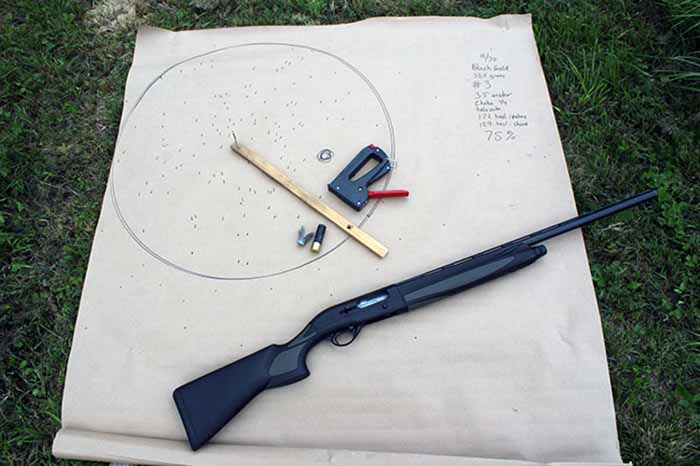
\includegraphics[width=0.7\textwidth]{Billeder/Andet/skudtest2.jpg}
        % Eller: [height=0.6\textheight] for højde-baseret skalering
    \end{center}
    
    % Her kan du tilføje tekst under billedet
    \vspace{1em}
    
\end{frame}




\begin{frame}{Jagtvåben typer}
    \begin{center}
        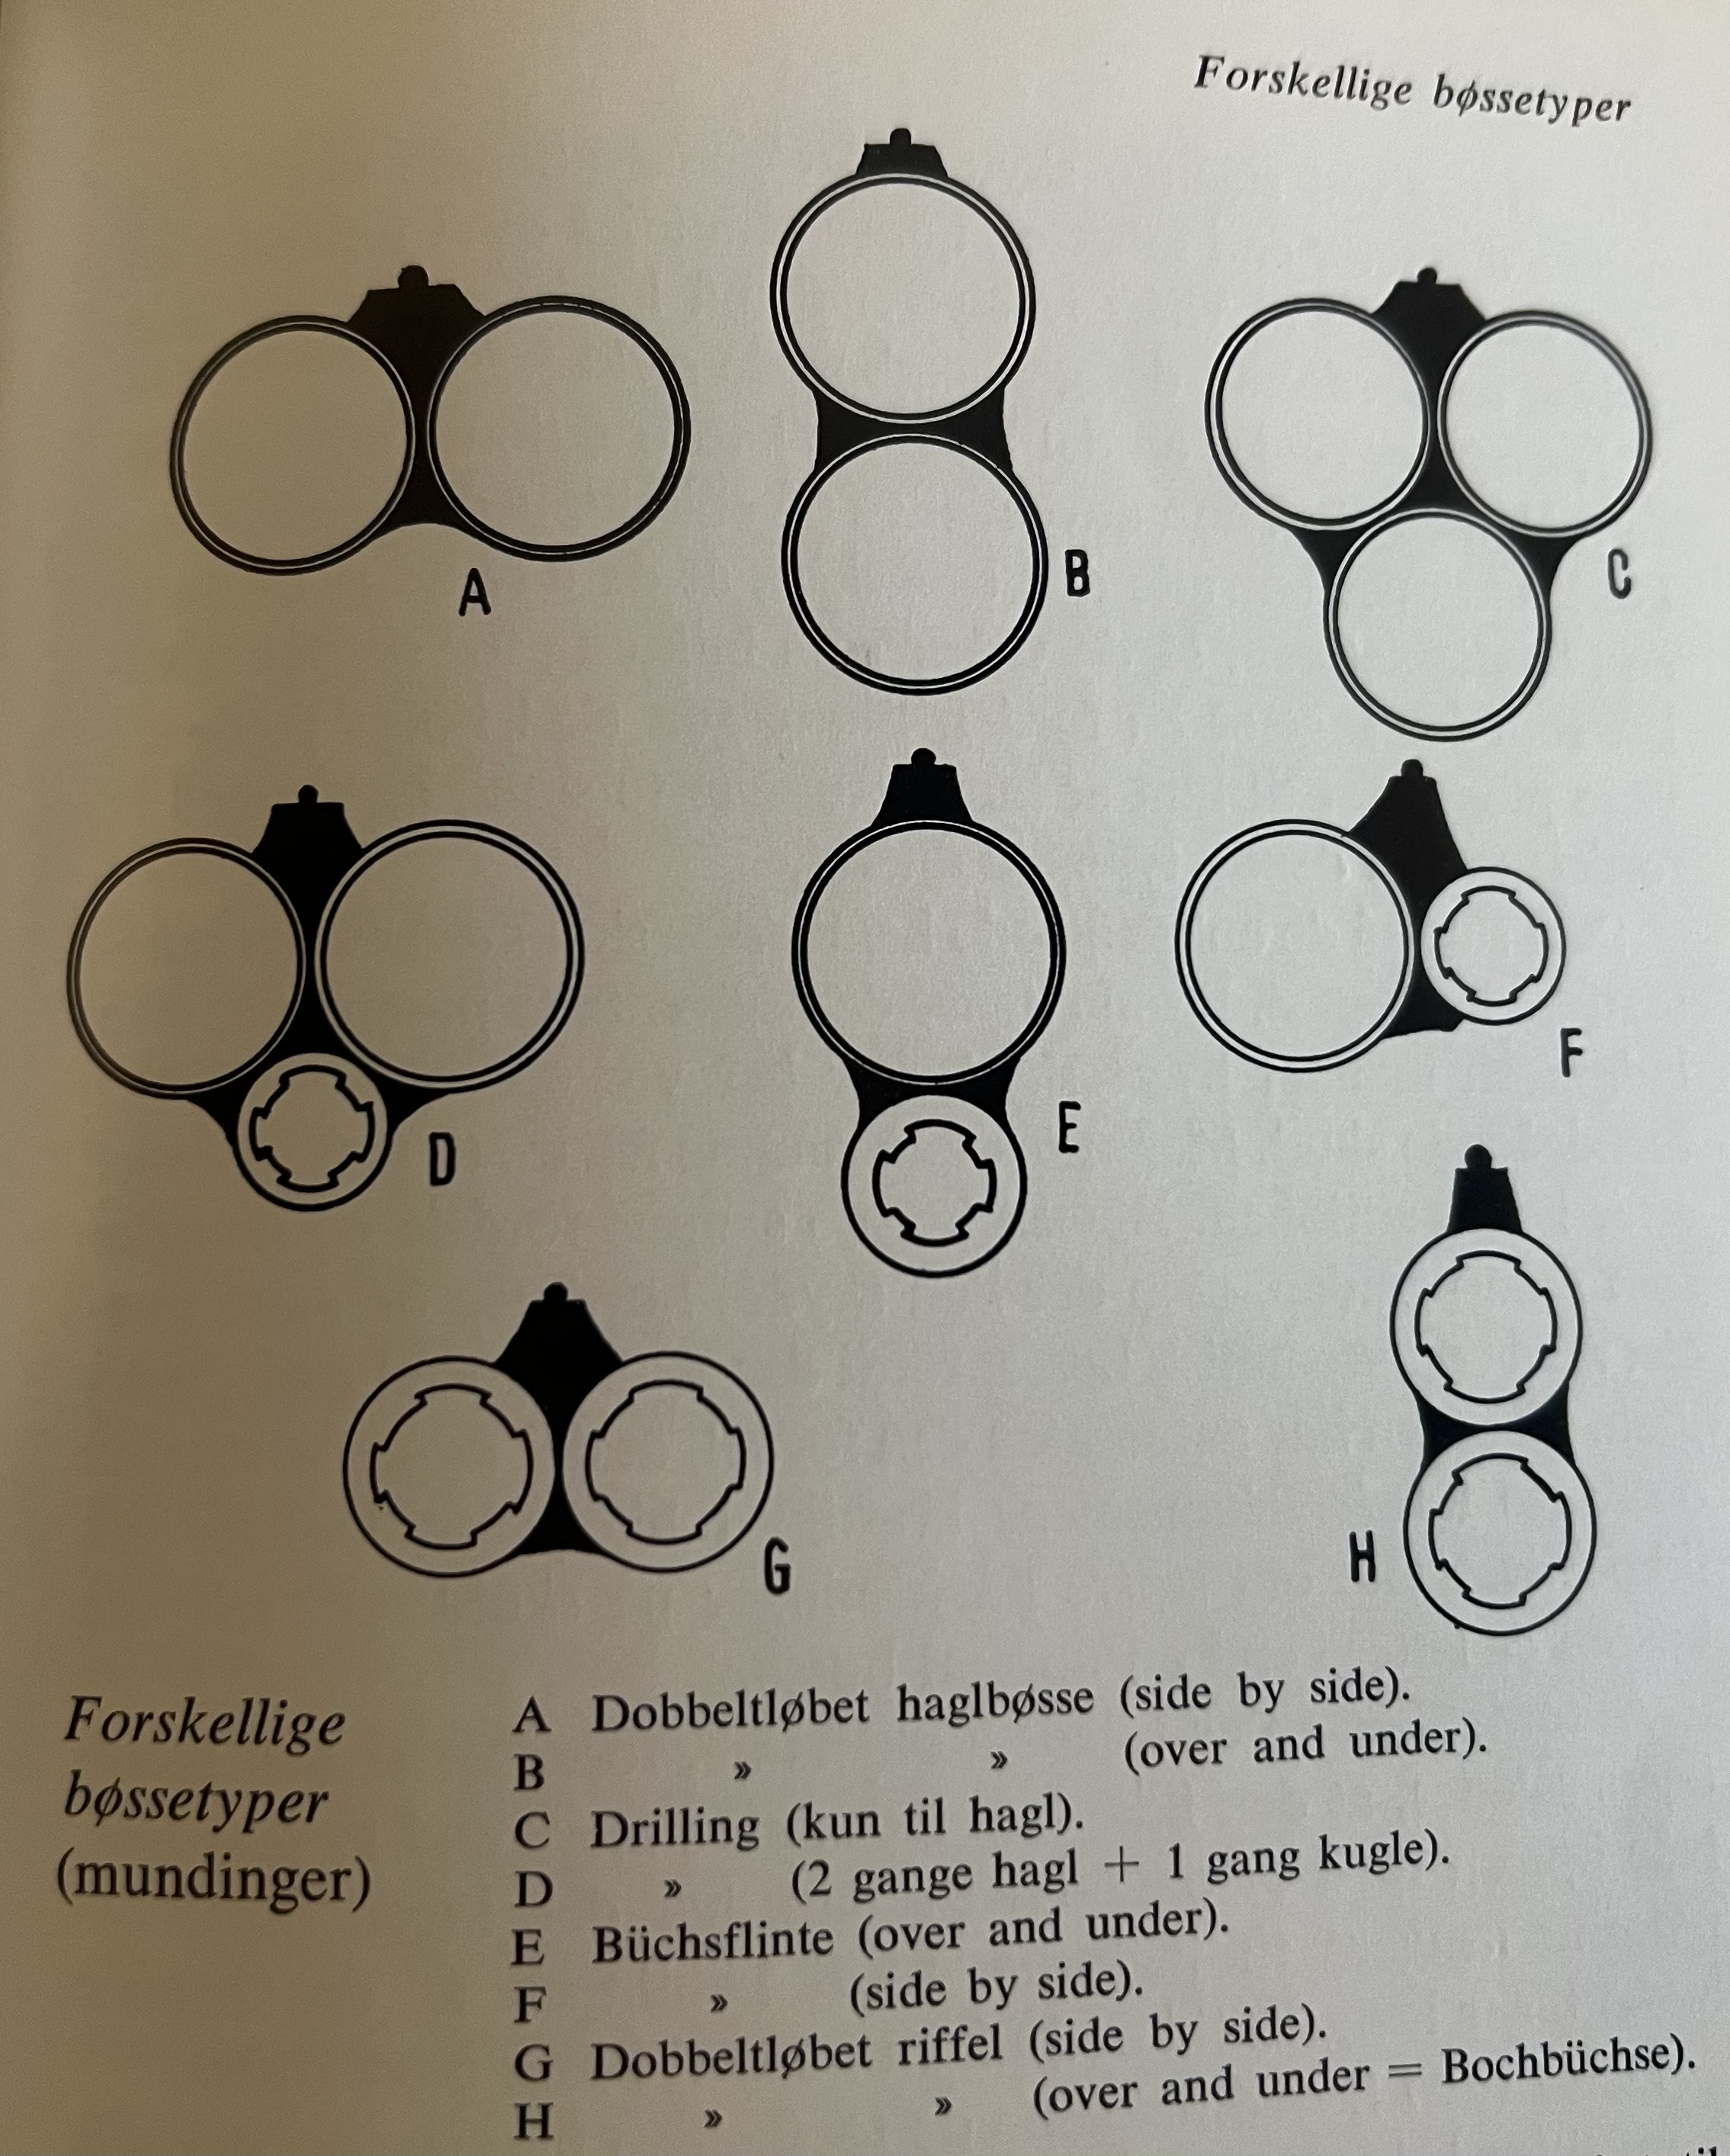
\includegraphics[width=0.3\textwidth]{Billeder/Andet/haglvarianter.jpeg}
        % Eller: [height=0.6\textheight] for højde-baseret skalering
    \end{center}
    
    % Her kan du tilføje tekst under billedet
    \vspace{1em}
    
\end{frame}

\begin{frame}{Haglvåben skæftetyper}
    \begin{center}
        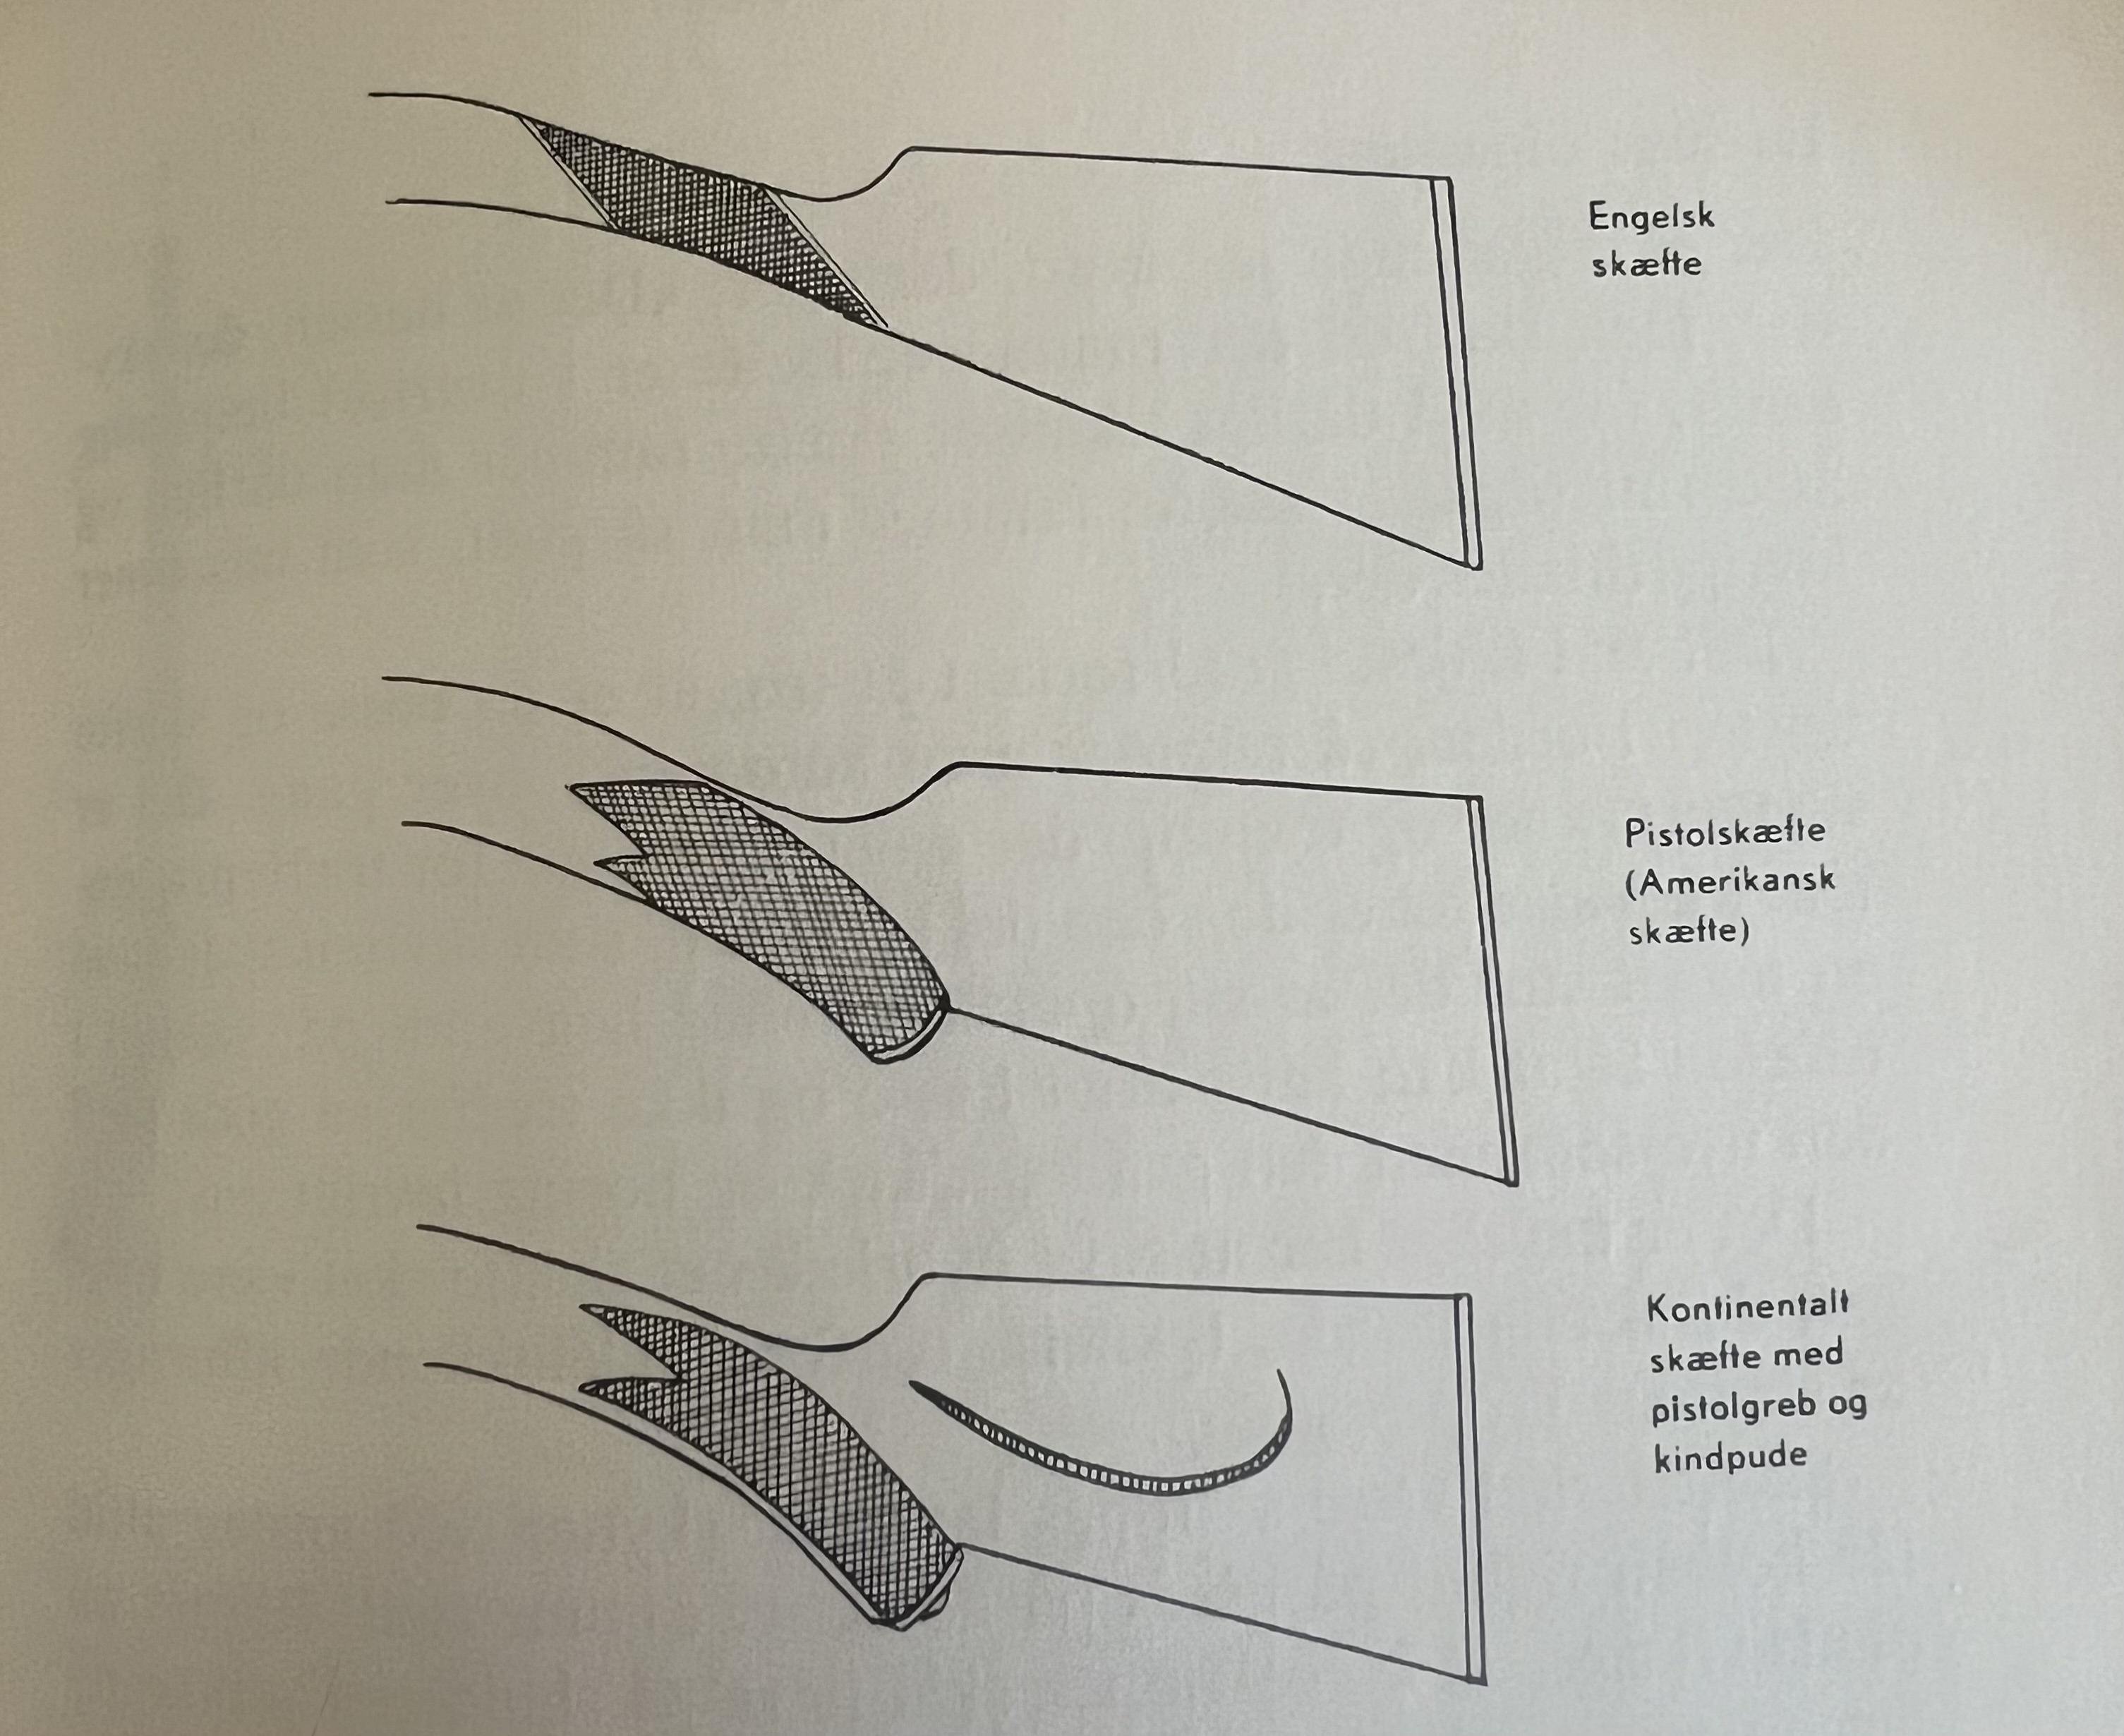
\includegraphics[width=0.5\textwidth]{Billeder/Andet/haglskaefter.jpeg}
        % Eller: [height=0.6\textheight] for højde-baseret skalering
    \end{center}
    
    % Her kan du tilføje tekst under billedet
    \vspace{1em}
    
\end{frame}

\begin{frame}{Haglvåben kalibre}
    \begin{center}
        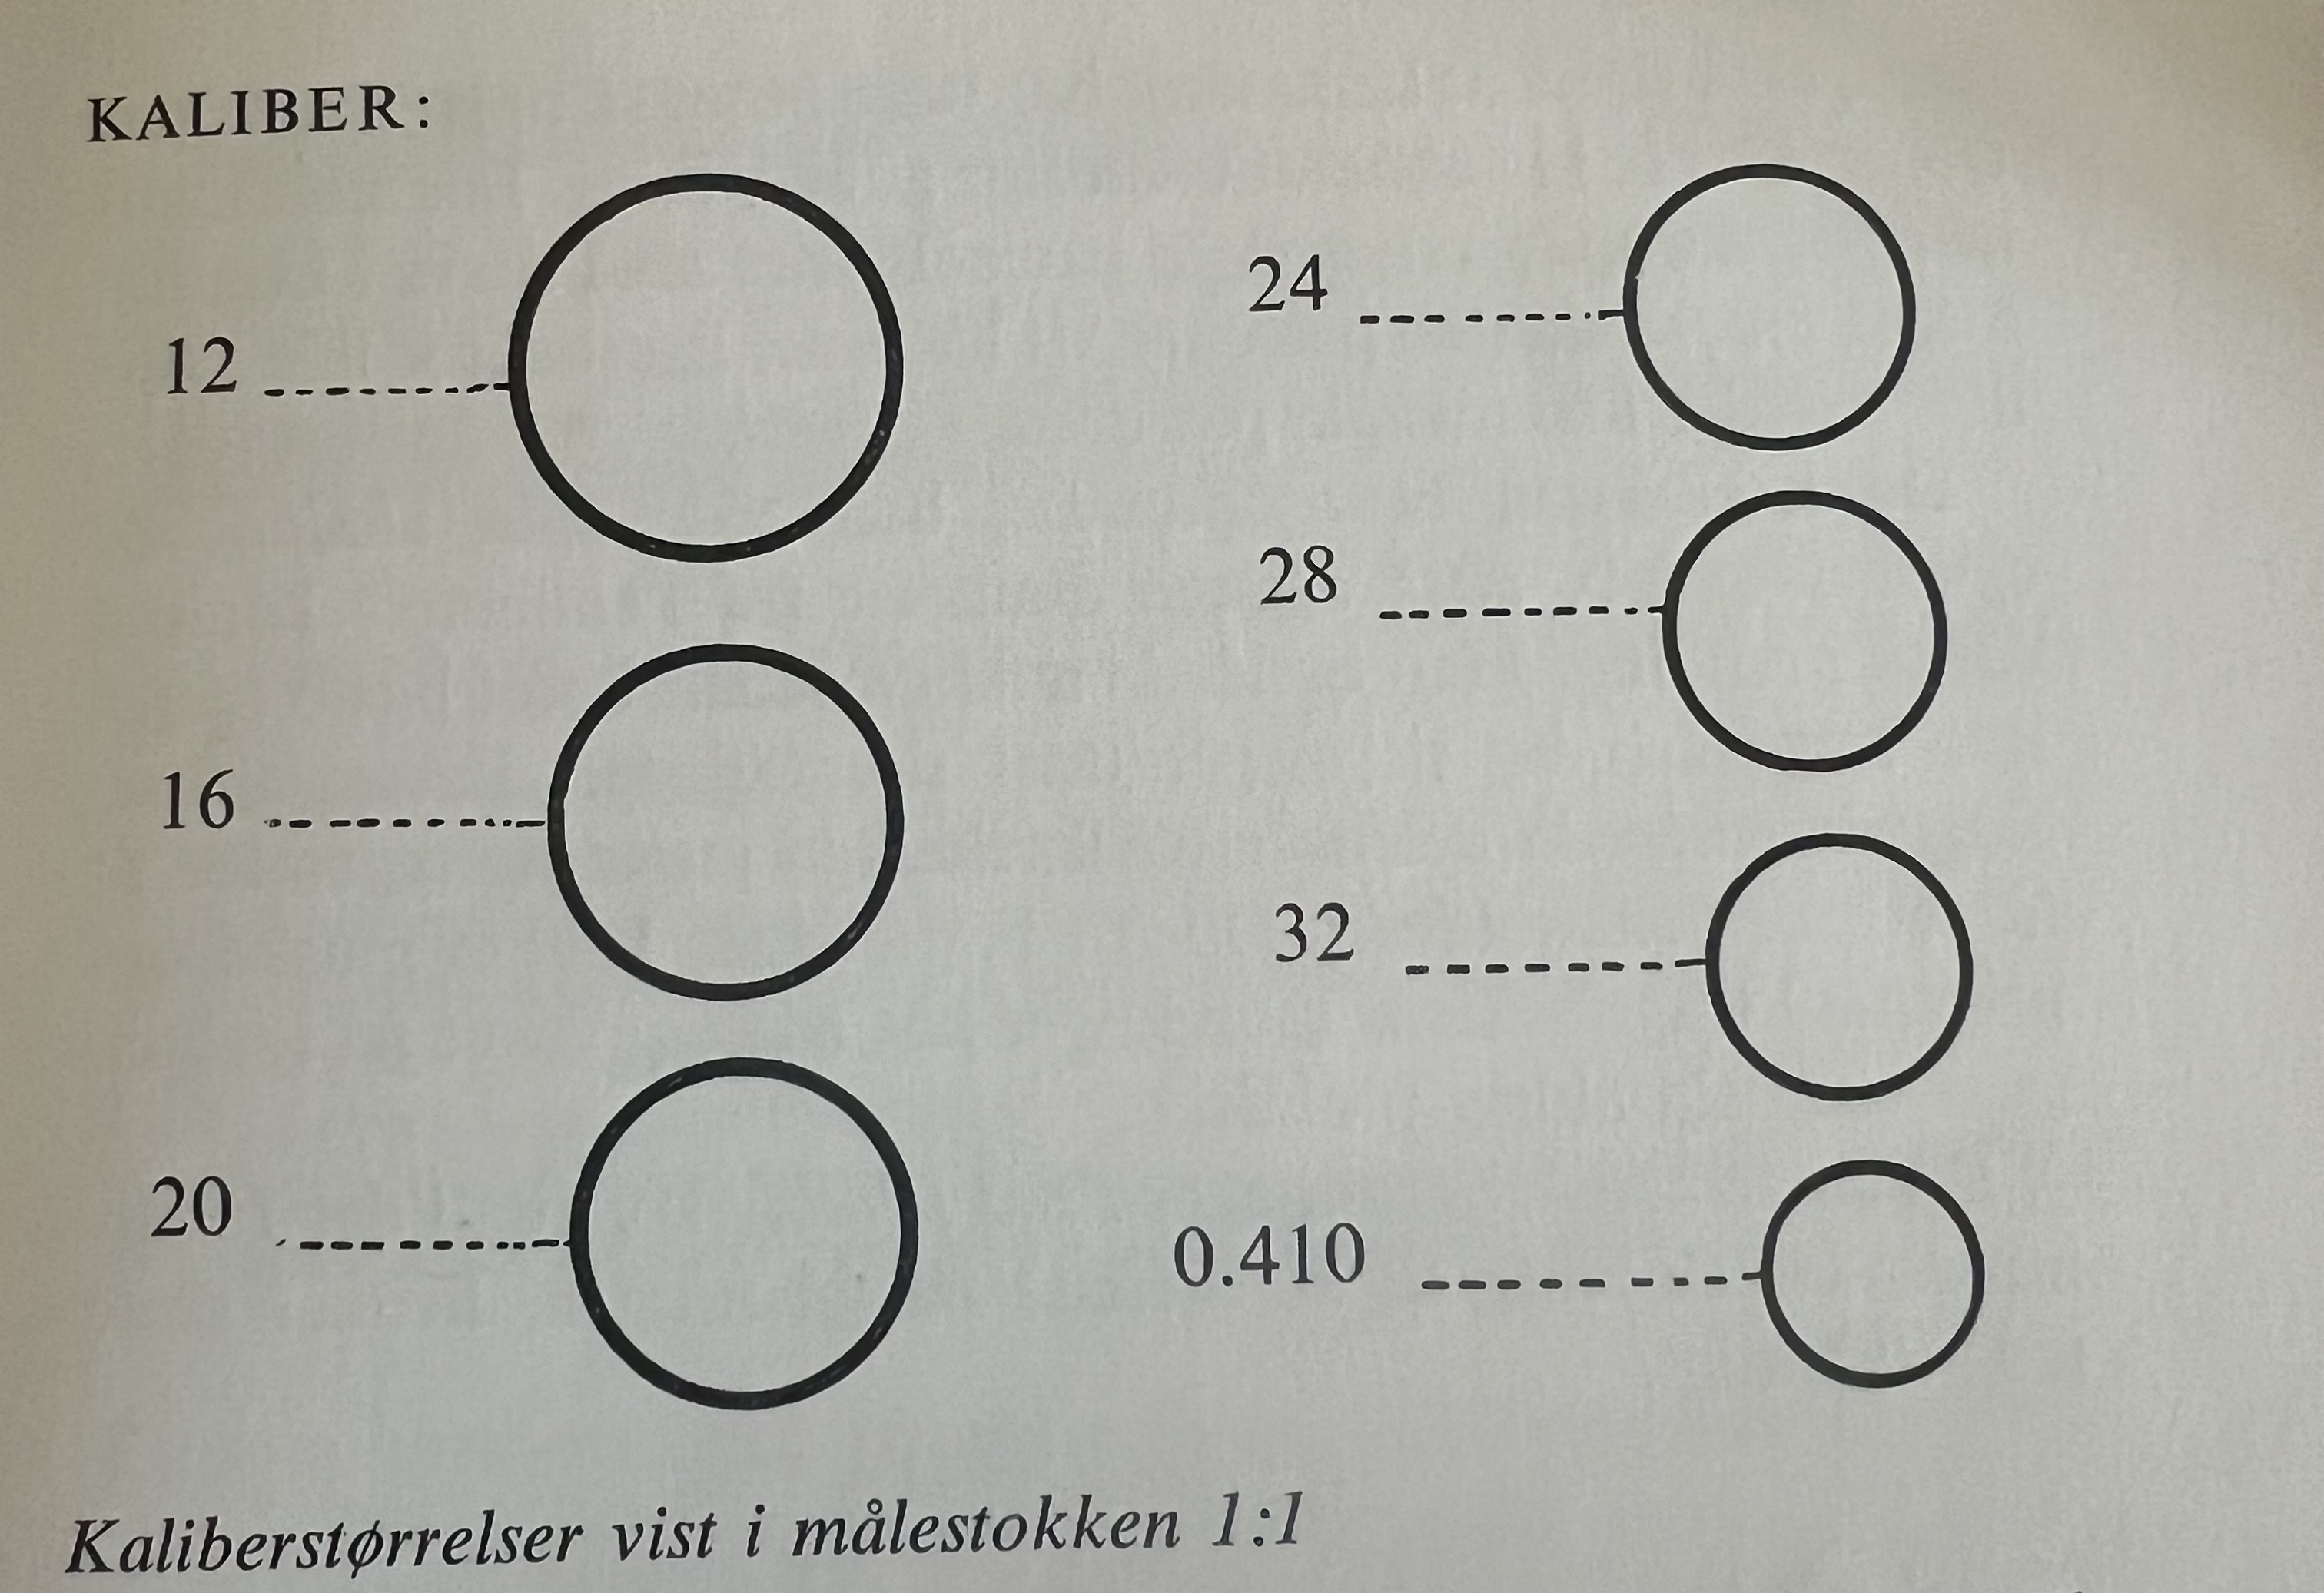
\includegraphics[width=0.5\textwidth]{Billeder/Andet/haglkalibre.jpeg}
        % Eller: [height=0.6\textheight] for højde-baseret skalering
    \end{center}
    
    % Her kan du tilføje tekst under billedet
    \vspace{1em}
    
\end{frame}

\begin{frame}{Sikkerhed med ammunition}
    \begin{itemize}
        \item Forkert kaliber til gevær (tilstopning)
        \item Håndtering af klikker (peg sikker retning, afvrid projektil)
    \end{itemize}
\end{frame}

\begin{frame}{Haglstørrelser og sikkerhedsafstand}
    \begin{center}
        \begin{tabular}{|c|c|c|}
            \hline
            
            \textbf{Nr.} & \textbf{Diameter (mm)} & \textbf{Sikkerhedsafstand (ca. ×100)} \\
            \hline
            Nr. 1 & 4,00 mm & 400 m \\
            Nr. 2 & 3,75 mm & 375 m \\
            Nr. 3 & 3,50 mm & 350 m \\
            Nr. 4 & 3,25 mm & 325 m \\
            Nr. 5 & 3,00 mm & 300 m \\
            Nr. 6 & 2,75 mm & 275 m \\
            Nr. 7 & 2,50 mm & 250 m \\
            \hline
        \end{tabular}
    \end{center}
    
    \vspace{1em}
    \small
    \textbf{Bemærk:} \\
    $\times 100$ er en meget grov tommelfingerregel for potentiel maksimal rækkevidde ved høj affyringsvinkel. \\
    Reelt: Nr. 1–2 hagl kan nå 200–300 m ved flad skud, men op til 400+ m ved stejl vinkel. \\
    Altid hold 200–300 m sikkerhedsafstand til veje, huse, mennesker mv. – uanset haglstørrelse!
\end{frame}

\begin{frame}{Sikkerhedsafstande riffel}
    \begin{itemize}
        \item Alm jagtriffel = 5000 m (5km)
        \item Salonriffel = 3000 m (3km)
    \end{itemize}
\end{frame}

\input{Frames/Jagtetik/Jagtudtryk/jagtudtryk_del_3}

\section{Repetition Teori 1-5}

\begin{frame}
  \vspace{3em}
  \begin{center}
    {\LARGE \textbf{Repetition: Teori 1-5 (Kahoot)}}
  \end{center}
\end{frame}

\section{Jagtformer}

\begin{frame}
  \vspace{3em}
  \begin{center}
    {\LARGE \textbf{Jagtformer}
    }
    \\
    \vspace{1em}
  \end{center}
\end{frame}


\begin{frame}{Pürsch}
    
    \begin{columns}[T]
        \begin{column}{0.58\textwidth}
            \begin{itemize}
                \item Jægeren opsøger vildtet \textbf{aktivt} i terrænet
                \item Bevægelse foregår \textbf{langsomt} og lydløst (ofte mod vinden)
                \item Stor vægt på \textbf{opsøgende evner} og viden om dyrets adfærd
                \item Ingen drivere eller standpladser
                \item Klassisk form for storvildtjagt (rådyr, kronvildt, dåvildt)
                \item Kræver god kondition og tålmodighed
                \item Der anvendes ikke hund til denne jagtform
                \item Der anvendes riffel, bue (ikke haglgevær)
            \end{itemize}
        \end{column}
        
        \begin{column}{0.4\textwidth}
            \centering
            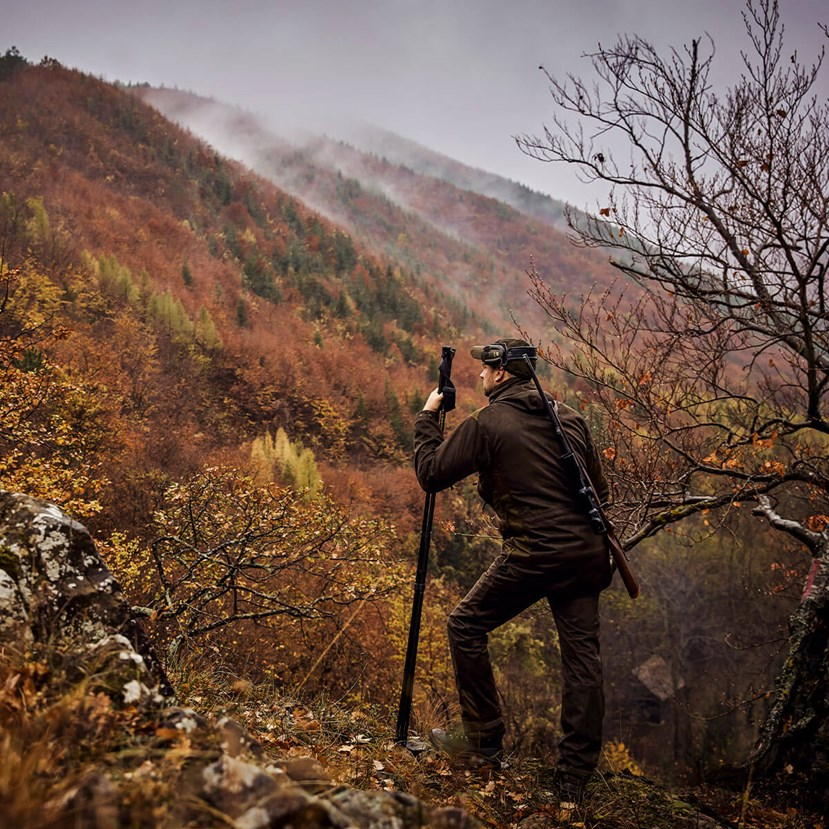
\includegraphics[width=\textwidth,height=0.85\textheight,keepaspectratio]
                {Billeder/Jagtformer/pursch}
            % Alternativt brug en af disse stilrene billeder:
            % \includegraphics[width=\textwidth]{highseat-snow-forest-hunter.jpg}
            % \includegraphics[width=\textwidth]{hunter-leaning-tree-rifle.jpg}
        \end{column}
    \end{columns}
    
\end{frame}


\begin{frame}{Trampejagt}
    
    \begin{columns}[T]
        \begin{column}{0.58\textwidth}
            \begin{itemize}
                \item Aktiv jagtform med mange deltagere
                \item Klassisk social og gammeldags jagtform
                \item Arealer drives af med jægere og drivere i tæt drev
                \item Der er ikke for- og bagposter placeret
                \item Der anvedes hunde med kort søg
                \item Der anvendes haglgevær
            \end{itemize}
        \end{column}
        
        \begin{column}{0.4\textwidth}
            \centering
            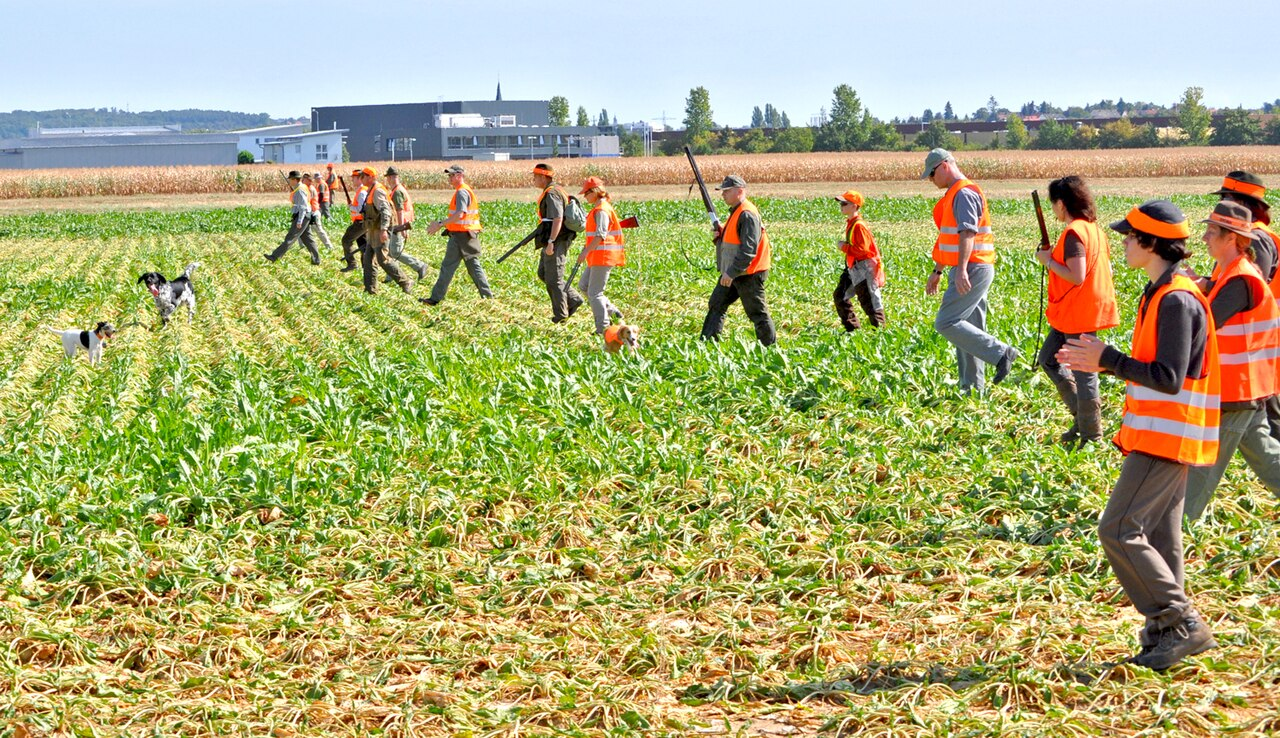
\includegraphics[width=\textwidth,height=0.85\textheight,keepaspectratio]
                {Billeder/Jagtformer/trampejagt_01}
            % Alternativt brug en af disse stilrene billeder:
            % \includegraphics[width=\textwidth]{highseat-snow-forest-hunter.jpg}
            % \includegraphics[width=\textwidth]{hunter-leaning-tree-rifle.jpg}
        \end{column}
    \end{columns}
    
\end{frame}


\begin{frame}{Trykjagt (bewegungsjagt)}
    
    \begin{columns}[T]
        \begin{column}{0.58\textwidth}
            \begin{itemize}
                \item Semi-aktiv jagtform med få drivere 
                \item Jægere placeres vilkårligt i terræn
                \item Få drivere skubber rundt til hovdyr
                \item Der anvendes riffel eller bue
                \item Der anvendes sjældent hunde i så fald meget kortsøgende eller i snor
                \item Dyrene kommer langsomt (=bedre skydning/afskydning))
                \item Jægere er typisk placeret i stiger, tårne eller treestand
            \end{itemize}
        \end{column}
        
        \begin{column}{0.4\textwidth}
            \centering
            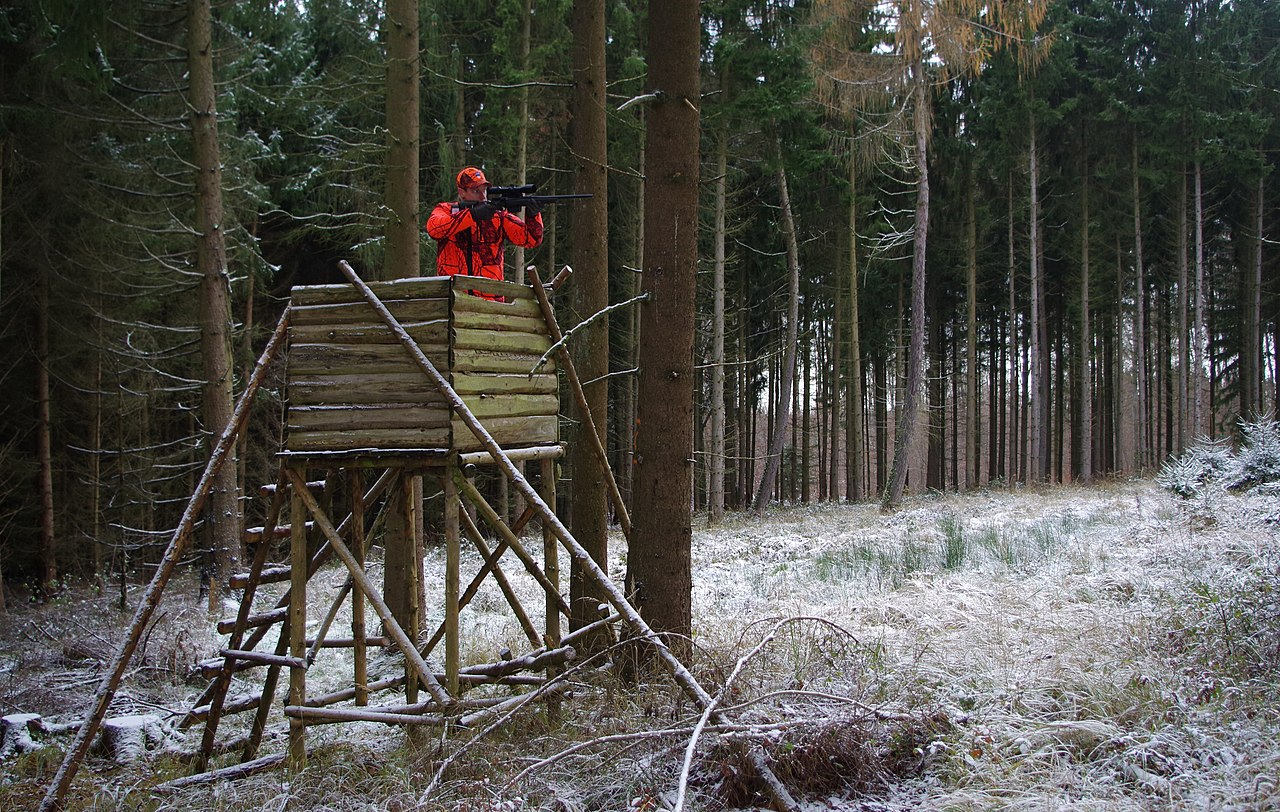
\includegraphics[width=\textwidth,height=0.85\textheight,keepaspectratio]
                {Billeder/Jagtformer/trykjagt_01}
            % Alternativt brug en af disse stilrene billeder:
            % \includegraphics[width=\textwidth]{highseat-snow-forest-hunter.jpg}
            % \includegraphics[width=\textwidth]{hunter-leaning-tree-rifle.jpg}
        \end{column}
    \end{columns}
    
\end{frame}

\begin{frame}{Drivjagt}
    
     \begin{columns}[T]
        \begin{column}{0.58\textwidth}
            \begin{itemize}
                \item \textbf{Semi-aktiv} jagtform – vildtet drives frem til jægerne
                \item Jægeren placeres rundt om området der drives
                \item Jægeren er typisk placeret i jagttårn el lign
                \item Vildtet kommer hurtigt
                \item Større krav til skydefærdigheder
                \item Alle våbentyper i brug
                \item Tæt systematisk drev (drevet går på linie)
                \item Anvendeligt på meget store arealer
                \item Anvendes langsomme jagthunde (terrier, beagle etc)
            \end{itemize}
        \end{column}
        
         \begin{column}{0.4\textwidth}
            \centering
            \vspace{0.5em}
            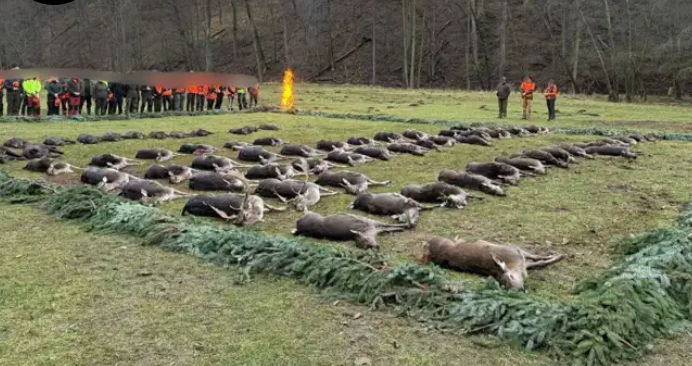
\includegraphics[width=\textwidth,height=0.82\textheight,keepaspectratio]
                {Billeder/Jagtformer/drivjagt}
            % Alternativer – fjern kommentartegn hvis du vil skifte:
            % \includegraphics[width=\textwidth]{highseat-snow-forest-hunter.jpg}
            % \includegraphics[width=\textwidth]{hunter-highseat-morning-mist.jpg}
            % \includegraphics[width=\textwidth]{ansitz-jagttarn-skov.jpg}
        \end{column}
    \end{columns}
    
\end{frame}

\begin{frame}{Anstandsjagt}
    
     \begin{columns}[T]
        \begin{column}{0.58\textwidth}
            \begin{itemize}
                \item \textbf{Passiv} jagtform – jægeren venter på vildtet
                \item Jægeren placerer sig strategisk i terrænet
                \item Foregår typisk fra: jagttårn, jagtstige, treestand
                \item Fordele:
                  \begin{itemize}
                    \item Kontrolleret og sikkert skud
                    \item God styr på vindretning
                    \item Vildtet forstyrres minimalt
                  \end{itemize}
                \item Vildtet drives ikke frem – det kommer naturligt
                \item Meget udbredt på hjortevildt (råvildt, dåvildt, kronvildt)
                \item Kræver tålmodighed, god placering og viden om vildtets færden
                \item Anvendes ikke hunde til denne jagtform
            \end{itemize}
        \end{column}
        
         \begin{column}{0.4\textwidth}
            \centering
            \vspace{0.5em}
            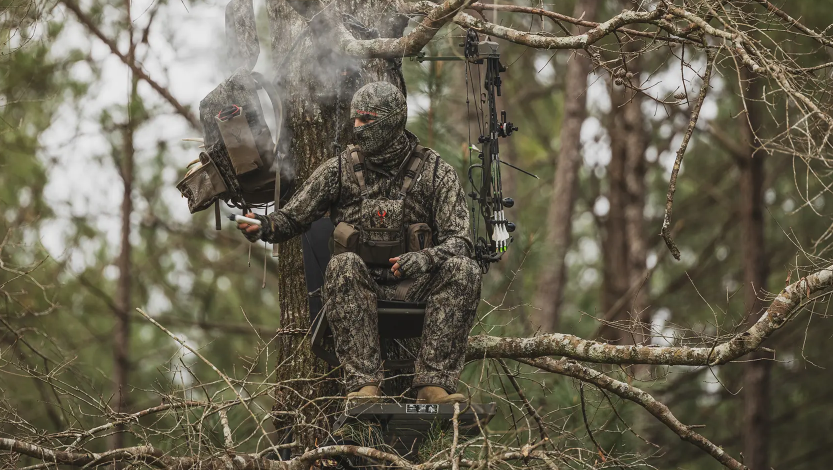
\includegraphics[width=\textwidth,height=0.82\textheight,keepaspectratio]
                {Billeder/Jagtformer/anstandsjagt.png}
            % Alternativer – fjern kommentartegn hvis du vil skifte:
            % \includegraphics[width=\textwidth]{highseat-snow-forest-hunter.jpg}
            % \includegraphics[width=\textwidth]{hunter-highseat-morning-mist.jpg}
            % \includegraphics[width=\textwidth]{ansitz-jagttarn-skov.jpg}
        \end{column}
    \end{columns}
    
\end{frame}


\begin{frame}{Trækjagt}
    
    \begin{columns}[T]
        \begin{column}{0.58\textwidth}
            \begin{itemize}
                \item Passiv jagtform - venter på trækkende fugle
                \item Solo eller få jægere sammen
                \item Der anvendes skjul, camouflage og lokkefugle
                \item Meget udbredt jagtform i DK
                \item Der anvendes haglgevær
                \item Der anvendes apporterende hunde (lovkrav)
            \end{itemize}
        \end{column}
        
        \begin{column}{0.4\textwidth}
            \centering
            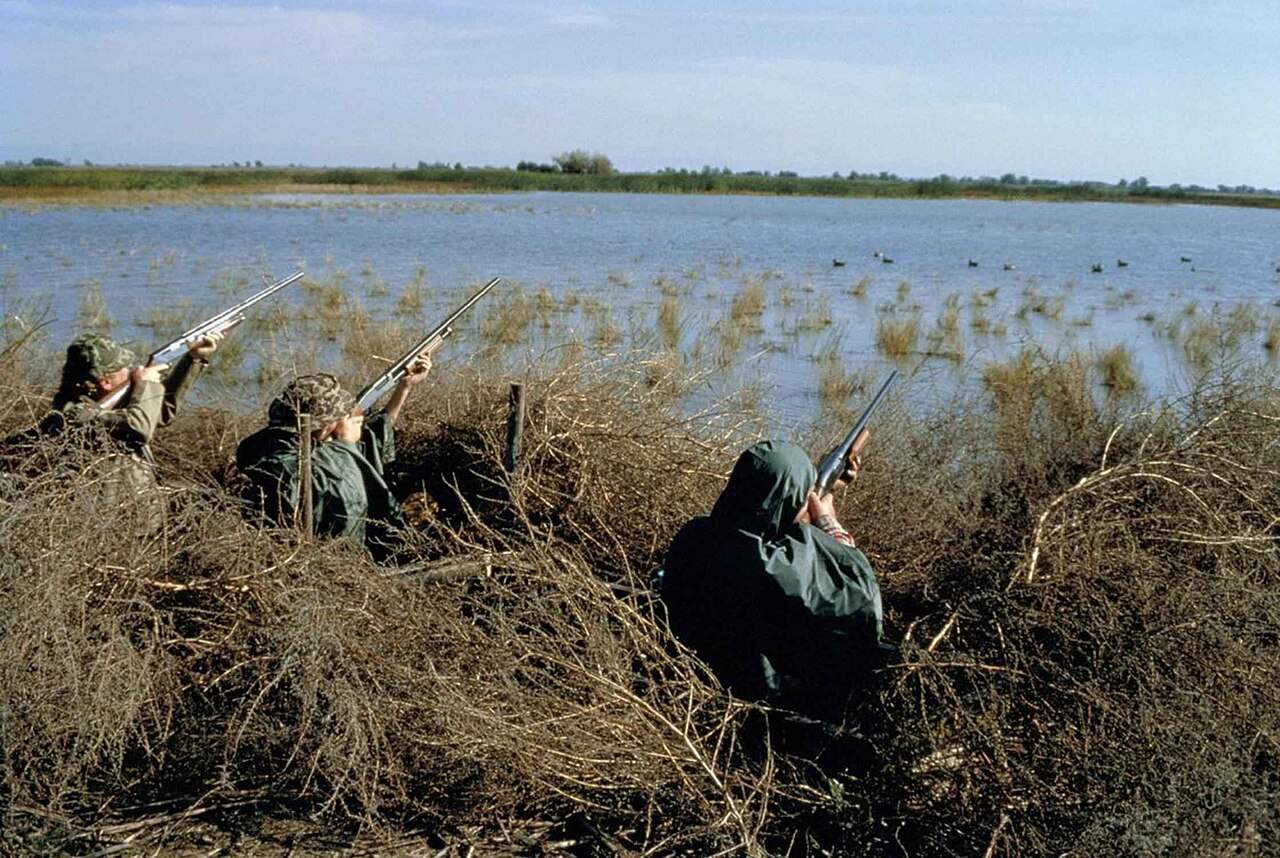
\includegraphics[width=\textwidth,height=0.85\textheight,keepaspectratio]
                {Billeder/Jagtformer/traekjagt_01}
            % Alternativt brug en af disse stilrene billeder:
            % \includegraphics[width=\textwidth]{highseat-snow-forest-hunter.jpg}
            % \includegraphics[width=\textwidth]{hunter-leaning-tree-rifle.jpg}
        \end{column}
    \end{columns}
    
\end{frame}


\begin{frame}{Strand- og havjagt}
    
    \begin{columns}[T]
        \begin{column}{0.58\textwidth}
            \begin{itemize}
                \item Pramjagt (passiv) - venter på trækkende fugle
                \item Motorbådsjagt (aktiv) - sejler med vinden mod fuglene
                \item Max hastighed 5 km/t under jagt
                \item Max hastighed 18 km/t før/efter jagt
                \item Gratis på fiskeriterritoriet
                \item Vær påpasselig med vejr, udstyr og sikkerhed
                \item Haglgevær anvendes
                \item Der anvendes typisk ikke hunde til jagtformen
            \end{itemize}
        \end{column}
        
        \begin{column}{0.4\textwidth}
            \centering
            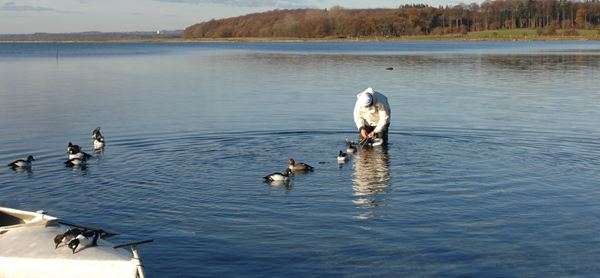
\includegraphics[width=\textwidth,height=0.85\textheight,keepaspectratio]
                {Billeder/Jagtformer/havjagt}
            % Alternativt brug en af disse stilrene billeder:
            % \includegraphics[width=\textwidth]{highseat-snow-forest-hunter.jpg}
            % \includegraphics[width=\textwidth]{hunter-leaning-tree-rifle.jpg}
        \end{column}
    \end{columns}
    
\end{frame}

\begin{frame}{Jagt for stående hund}
    
     \begin{columns}[T]
        \begin{column}{0.58\textwidth}
            \begin{itemize}
                \item \textbf{Aktiv} jagtform – hund med stort søg står stand ved typisk hønsefugl
                \item Typisk solo eller få jægere
                \item Jægeren giver signal til hunden om at lette fuglen ved stand
                \item Der anvendes glatløbet haglgevær til jagtformen
                \item Uddøende jagtform i DK pga. den intensive arealudnyttelse
            \end{itemize}
        \end{column}
        
         \begin{column}{0.4\textwidth}
            \centering
            \vspace{0.5em}
            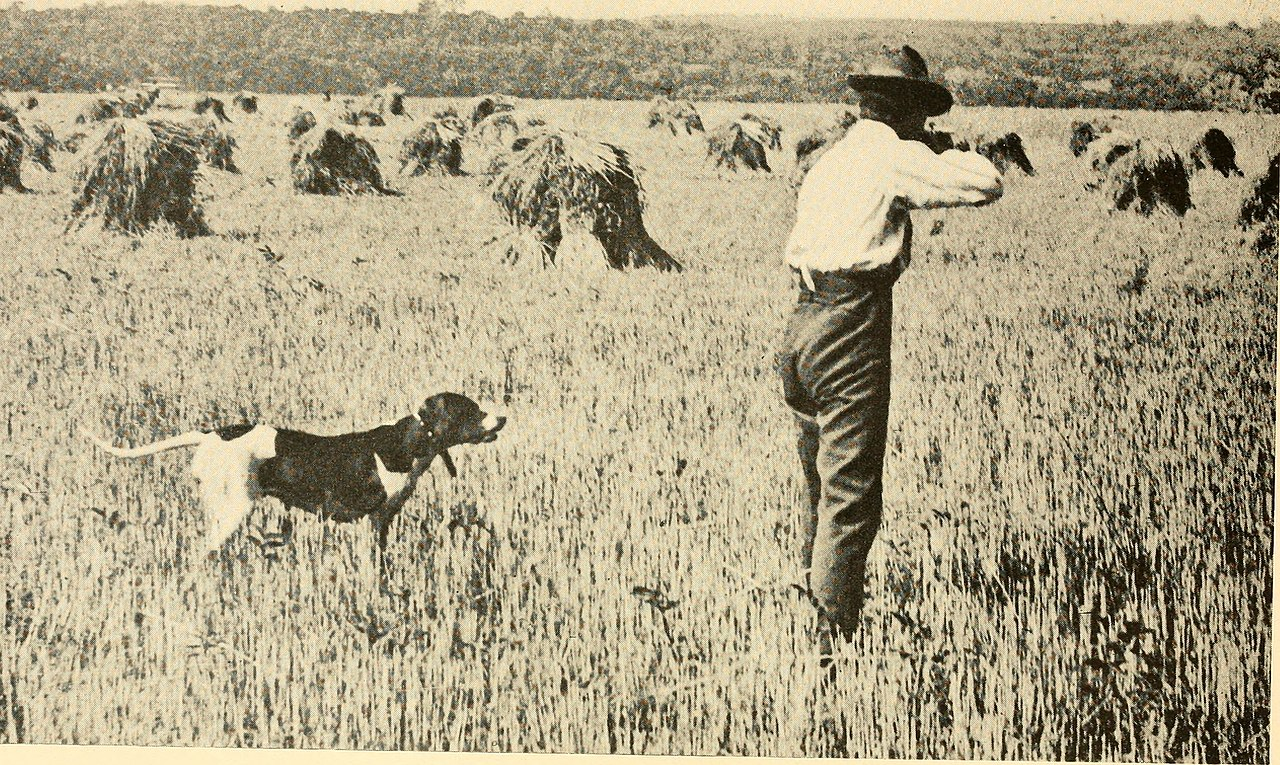
\includegraphics[width=\textwidth,height=0.82\textheight,keepaspectratio]
                {Billeder/Jagtformer/staaende_jagt}
            % Alternativer – fjern kommentartegn hvis du vil skifte:
            % \includegraphics[width=\textwidth]{highseat-snow-forest-hunter.jpg}
            % \includegraphics[width=\textwidth]{hunter-highseat-morning-mist.jpg}
            % \includegraphics[width=\textwidth]{ansitz-jagttarn-skov.jpg}
        \end{column}
    \end{columns}
    
\end{frame}





\begin{frame}{Jagt for stødende hund (rough shooting)}
    
     \begin{columns}[T]
        \begin{column}{0.58\textwidth}
            \begin{itemize}
                \item \textbf{Aktiv} jagtform – hund med kort søg letter vildtet som typisk nedlægges i bagskud 
                \item Typisk solo eller få jægere
                \item Der anvendes glatløbet haglgevær til jagtformen
                \item Udbredt jagtform i DK - passer til små arealer
            \end{itemize}
        \end{column}
        
         \begin{column}{0.4\textwidth}
            \centering
            \vspace{0.5em}
            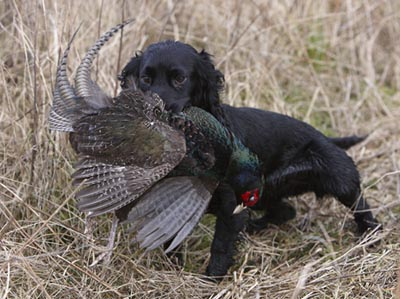
\includegraphics[width=\textwidth,height=0.82\textheight,keepaspectratio]
                {Billeder/Jagtformer/stoedende_01}
            % Alternativer – fjern kommentartegn hvis du vil skifte:
            % \includegraphics[width=\textwidth]{highseat-snow-forest-hunter.jpg}
            % \includegraphics[width=\textwidth]{hunter-highseat-morning-mist.jpg}
            % \includegraphics[width=\textwidth]{ansitz-jagttarn-skov.jpg}
        \end{column}
    \end{columns}
    
\end{frame}

\begin{frame}{Gravjagt}
    
     \begin{columns}[T]
        \begin{column}{0.58\textwidth}
            \begin{itemize}
                \item \textbf{Aktiv} jagtform – ræv jages ud af graven med gravsøgende hunde
                \item Jægerne placerer sig ved udgangene til gravsystemet
                \item Der anvendes glatløbet haglgevær til jagtformen
                \item Frivillige certificeringer af egnede hunde (gravhund/jack russell o.lign)
            \end{itemize}
        \end{column}
        
         \begin{column}{0.4\textwidth}
            \centering
            \vspace{0.5em}
            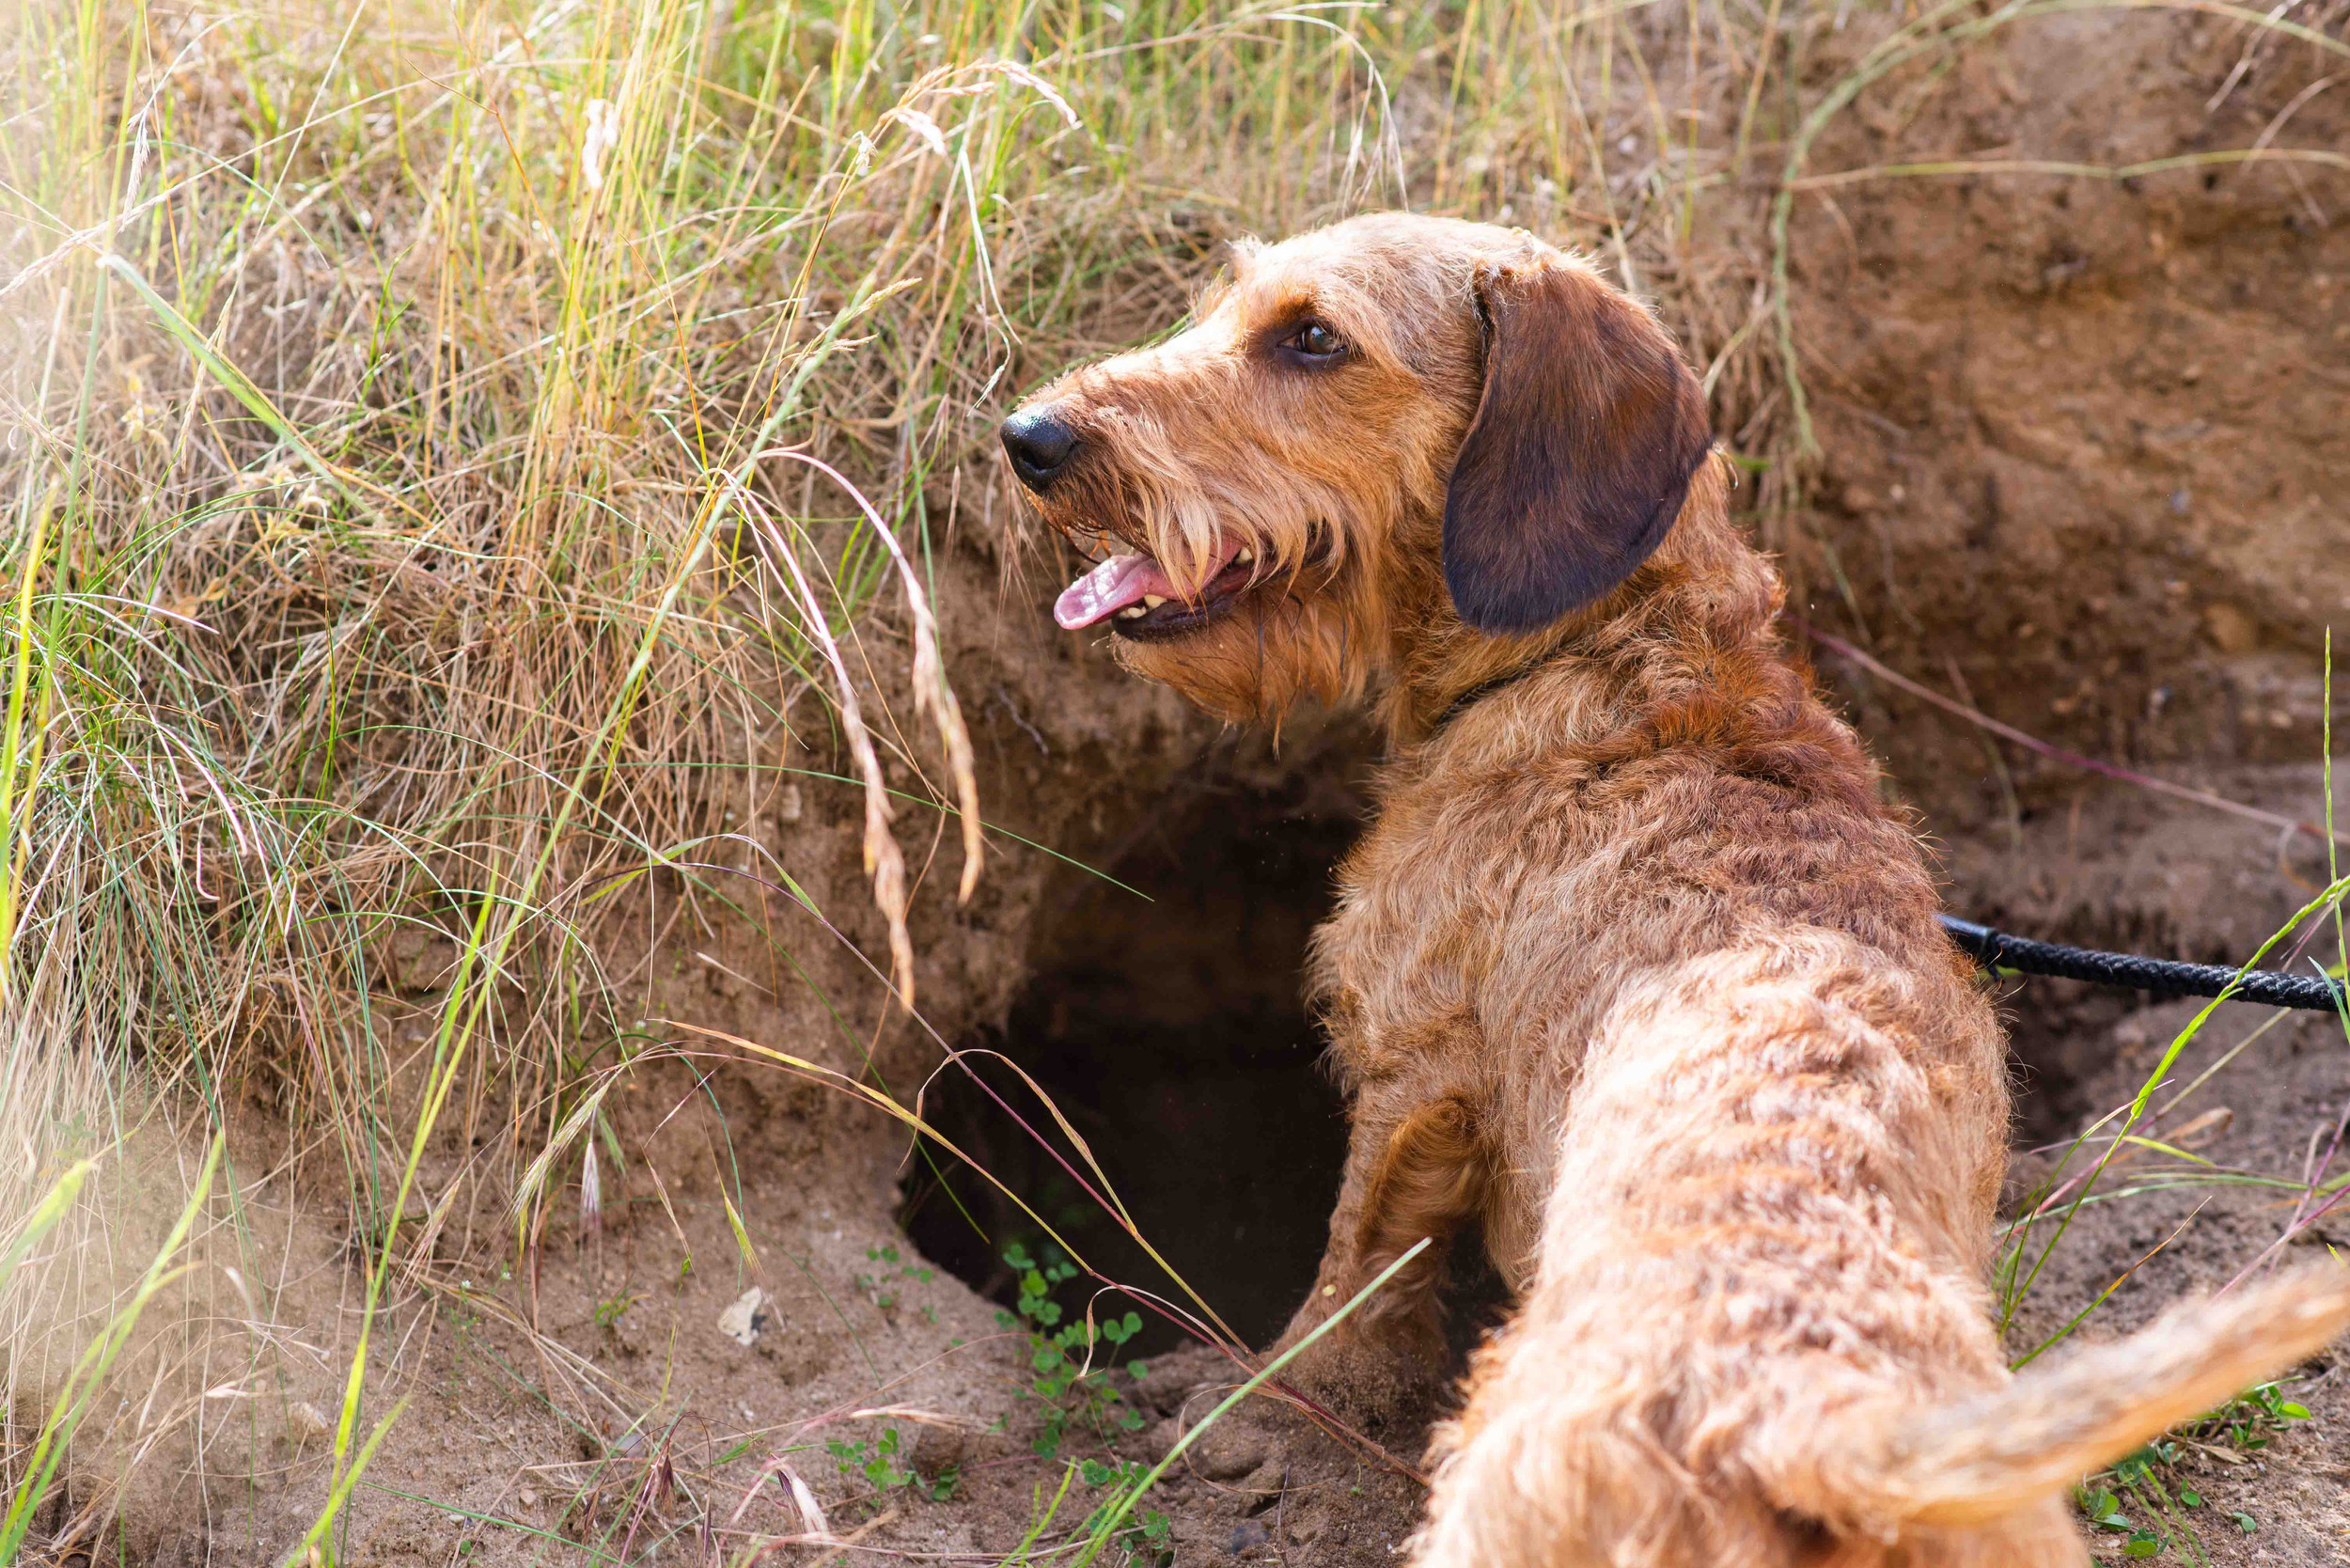
\includegraphics[width=\textwidth,height=0.82\textheight,keepaspectratio]
                {Billeder/Jagtformer/gravjagt}
            % Alternativer – fjern kommentartegn hvis du vil skifte:
            % \includegraphics[width=\textwidth]{highseat-snow-forest-hunter.jpg}
            % \includegraphics[width=\textwidth]{hunter-highseat-morning-mist.jpg}
            % \includegraphics[width=\textwidth]{ansitz-jagttarn-skov.jpg}
        \end{column}
    \end{columns}
    
\end{frame}

\section{Jagthunde}

\begin{frame}
  \vspace{3em}
  \begin{center}
    {\LARGE \textbf{Jagthunde}
    }
    \\
    \vspace{1em}
  \end{center}
\end{frame}

\begin{frame}{Bekendtgørelse af lov om jagt og vildtforvaltning § 24} % Lige justering af titlen
\vspace{1em}
\begin{columns}[c] % c = center vertically
\column{0.05\textwidth} % Venstre margin
\column{0.7\textwidth} % Midten: Bullets
\small
\raggedright
\begin{itemize}
\itemsep0.6em % Justér afstand mellem bullets
\item § 24. Ved jagt med glatløbet haglgevær på ikkeklovbærende vildt på og fra landarealer og i rør- og sivbevoksninger skal egnet apporterende hund medbringes.
\end{itemize}
\column{0.25\textwidth} % Højre: Ikon
\centering
\vspace{0pt}
% Der skal formentlig indsættes et passende billede/ikon her
\end{columns}
\end{frame}

\begin{frame}{Overordnede kategorier af jagthunde}

\vspace{1em}

\begin{columns}[c] % c = center vertically

\column{0.05\textwidth} % Venstre margin

\column{0.7\textwidth} % Midten: Bullets

\small

\raggedright

\begin{itemize}

\itemsep0.6em % Justér afstand mellem bullets

\item \textbf{Stående} (f.eks. Irsk Setter)
\item \textbf{Stødende} (f.eks. Cocker Spaniel)
\item \textbf{Apporterende} (f.eks. Labrador, Golden Retriever)
\item \textbf{Gravsøgende} (f.eks. Gravhund)
\item \textbf{Støvende (drivende)} (f.eks. Beagle)
\item \textbf{Schweisshunde} (f.eks. Blodhund)

\end{itemize}

\column{0.25\textwidth} % Højre: Ikon

\centering

\vspace{0pt}

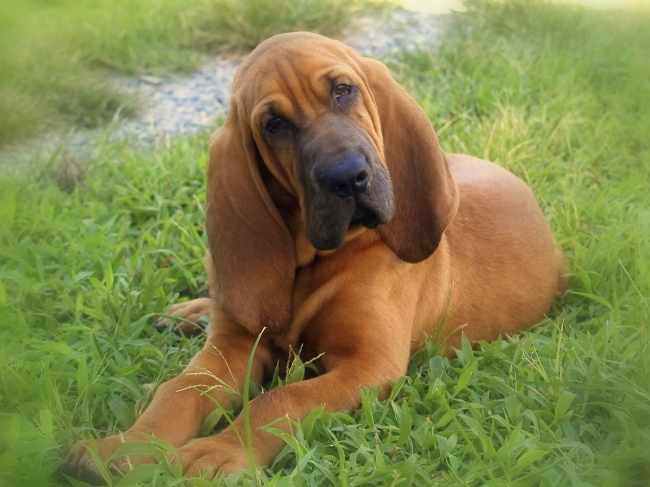
\includegraphics[width=0.9\linewidth]{Billeder/Jagthunde/schweisshunde/blodhund.jpg} % Ændret ikon til at passe med 'Hunde'

\end{columns}

\end{frame}

\begin{frame}{Apporterende jagthunde}

\vspace{1em}

\begin{columns}[c] % c = center vertically

\column{0.05\textwidth} % Venstre margin

\column{0.7\textwidth} % Midten: Bullets

\small

\raggedright

\begin{itemize}

\itemsep0.6em % Justér afstand mellem bullets

\item Hovedopgaven er at \textbf{finde og bringe nedlagt vildt} til jægeren (apportere).
\item Skal være \textbf{skudfast} og have en \textbf{blød mund} for ikke at ødelægge vildtet.
\item Er nødvendig ved jagt med haglgevær på ikke-klovbærende vildt på landarealer (§ 24).
\item Er ofte velegnede \textbf{familiehunde} grundet deres samarbejdsvilje.
\item \textbf{Racer}: Labrador Retriever, Golden Retriever, Flatcoated Retriever, Chesapeake Bay Retriever.

\end{itemize}

\column{0.25\textwidth} % Højre: Ikon

\centering

\vspace{0pt}

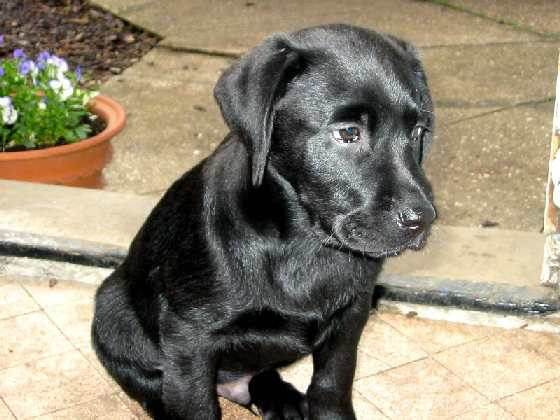
\includegraphics[width=0.9\linewidth]{Billeder/Jagthunde/apporterende/labrador.jpg} % Ikon af apporterende hund

\end{columns}

\end{frame}

\begin{frame}{Stødende jagthunde}

\vspace{1em}

\begin{columns}[c] % c = center vertically

\column{0.05\textwidth} % Venstre margin

\column{0.7\textwidth} % Midten: Bullets

\small

\raggedright

\begin{itemize}

\itemsep0.6em % Justér afstand mellem bullets

\item Hundens opgave er at \textbf{søge under bøssen} (tæt på jægeren) og rejse vildtet.
\item De skal "støde" vildtet, dvs. få det til at \textbf{flyve eller løbe op} inden for skudafstand.
\item Har typisk en \textbf{kort rækkevidde} i søget og arbejder tæt sammen med jægeren.
\item Bruges primært til jagt på \textbf{fugle} (f.eks. fasaner og ænder) og \textbf{kaniner}.
\item \textbf{Racer}: Cocker Spaniel, Springer Spaniel, Field Spaniel, Kleiner Münsterländer (kan også stå).

\end{itemize}

\column{0.25\textwidth} % Højre: Ikon

\centering

\vspace{0pt}

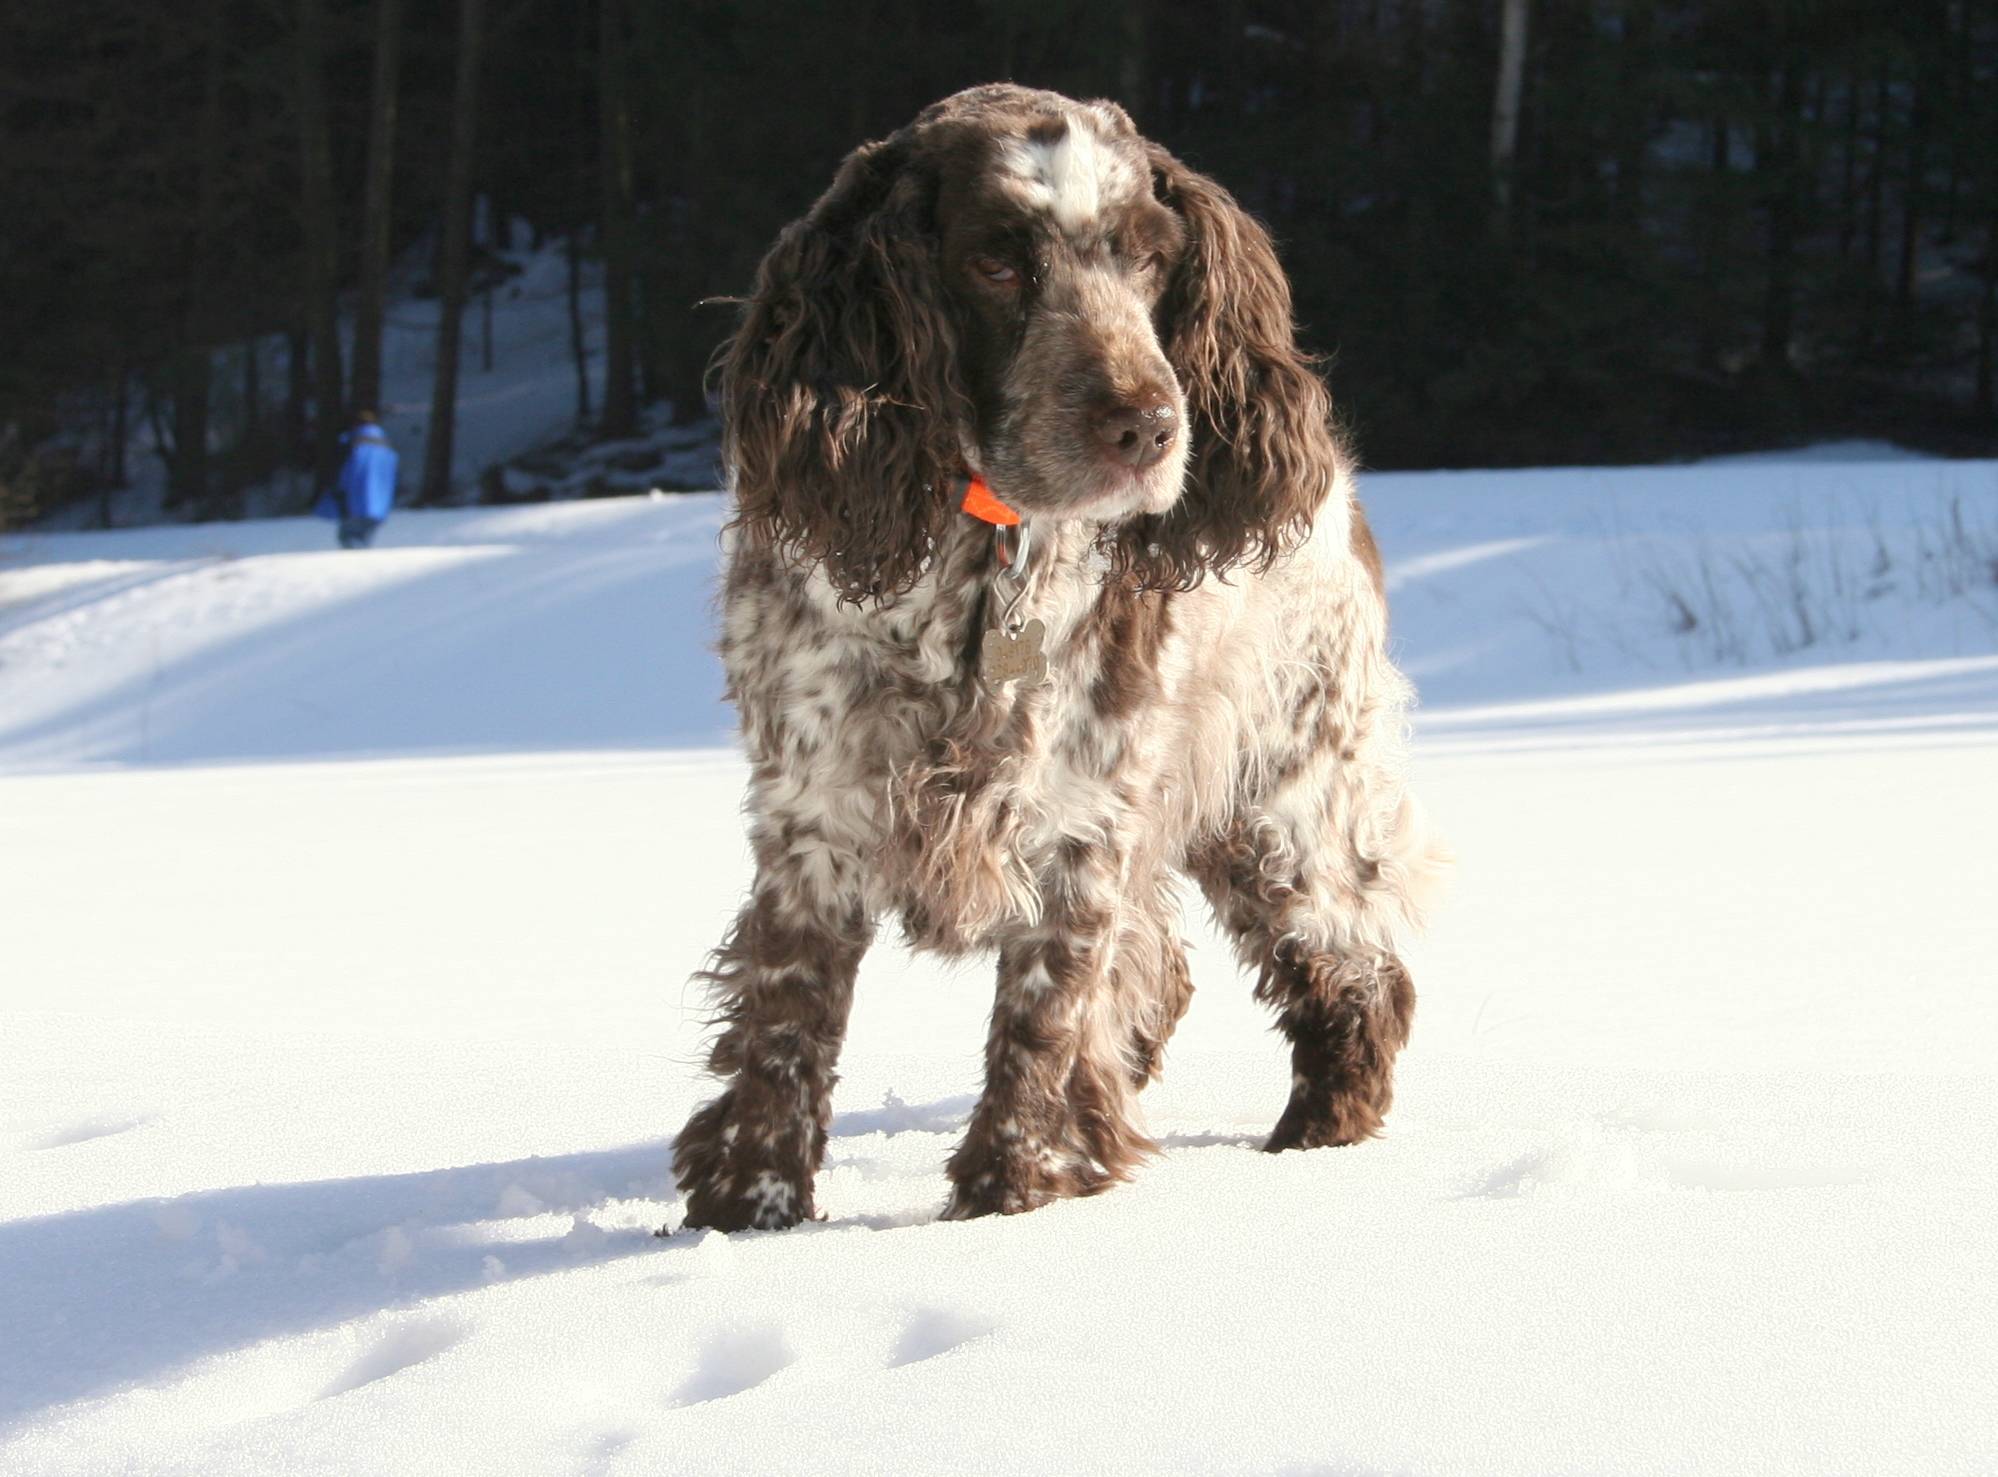
\includegraphics[width=0.9\linewidth]{Billeder/Jagthunde/stoedende/cocker.jpg} % Ikon af en spaniel i aktion

\end{columns}

\end{frame}

\begin{frame}{Stående jagthunde}

\vspace{1em}

\begin{columns}[c] % c = center vertically

\column{0.05\textwidth} % Venstre margin

\column{0.7\textwidth} % Midten: Bullets

\small

\raggedright

\begin{itemize}

\itemsep0.6em % Justér afstand mellem bullets

\item Udfører et \textbf{langt søg} i terrænet.
\item God til jagt i områder med \textbf{stor vildtspredning}.
\item Deres kendetegn er at \textbf{tage stand} for fuglevildt (pege). 
\item Opdeles primært i to typer: \textbf{Engelsk} (f.eks. Pointer, Setter) og \textbf{Kontinental} (f.eks. Ruhåret Hønsehund).
\item Anvendes til jagt på hønsefugle - jagtformen er aftagende.
\item \textbf{Racer}: Hønsehunde, Pointere, Settere, Wizla, Münsterländere, Breton, Weimaraner

\end{itemize}

\column{0.25\textwidth} % Højre: Ikon

\centering

\vspace{0pt}

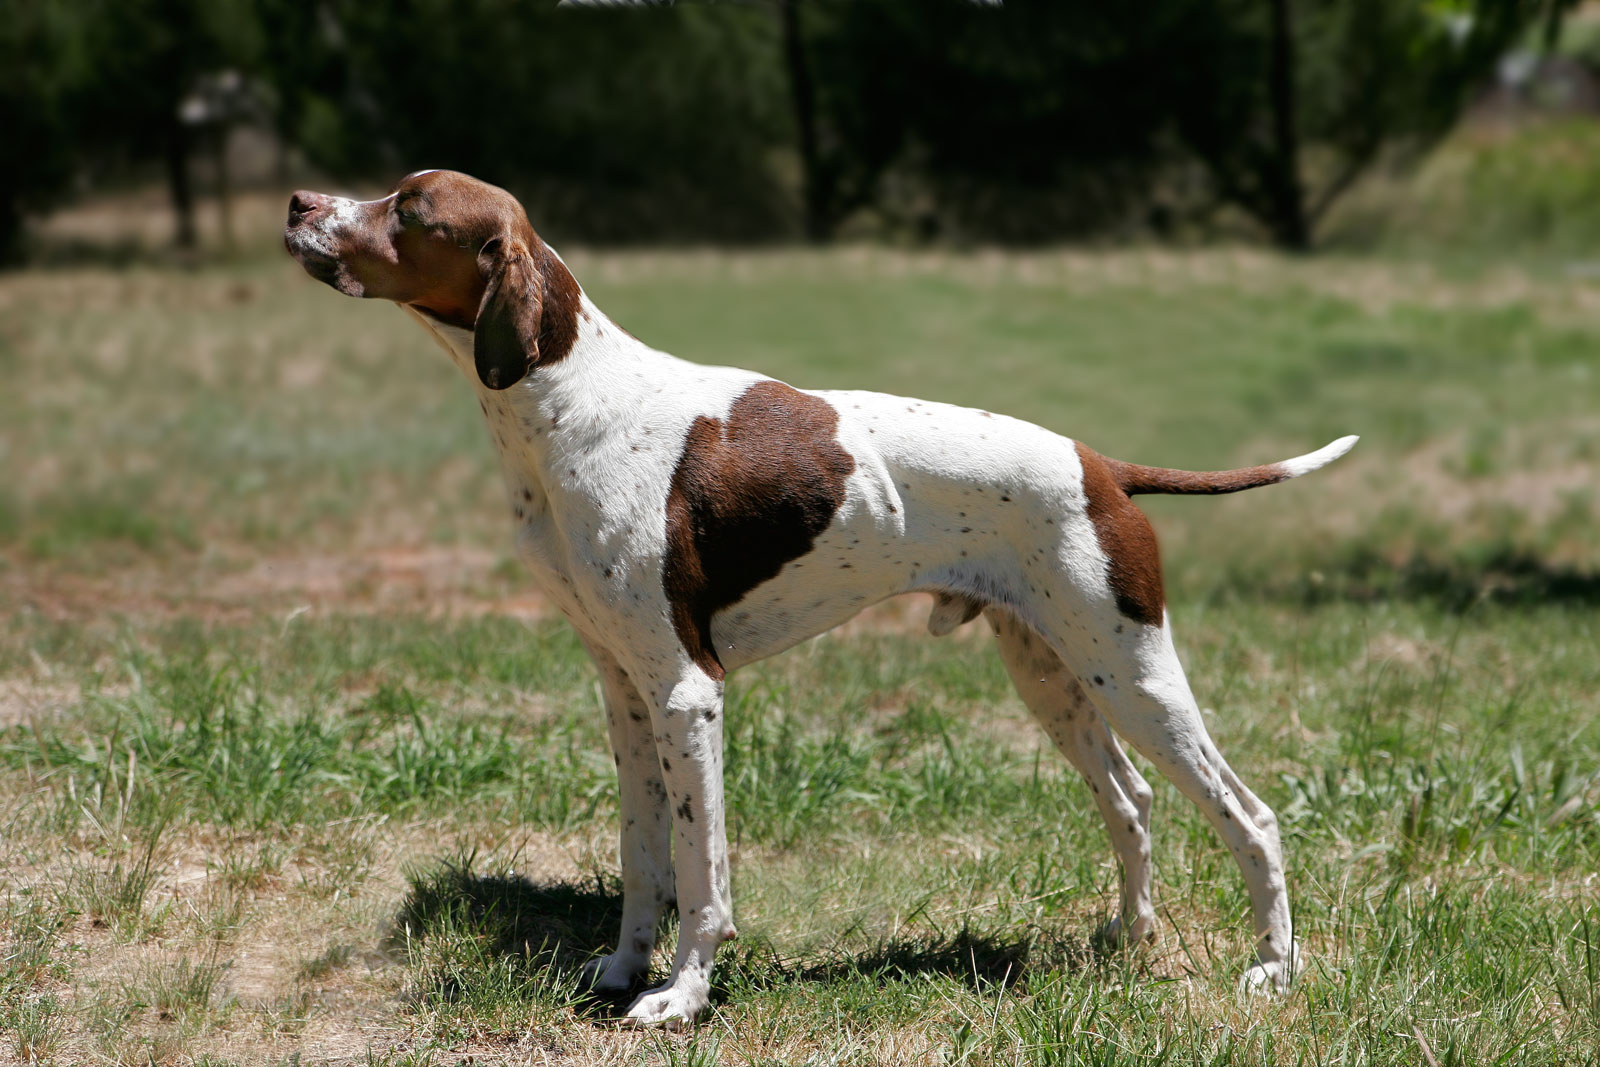
\includegraphics[width=0.9\linewidth]{Billeder/Jagthunde/staaende/English_pointer.jpg} % Ikon af stående hund

\end{columns}

\end{frame}

\begin{frame}{Støvende (Drivende) jagthunde}

\vspace{1em}

\begin{columns}[c] % c = center vertically

\column{0.05\textwidth} % Venstre margin

\column{0.7\textwidth} % Midten: Bullets

\small

\raggedright

\begin{itemize}

\itemsep0.6em % Justér afstand mellem bullets

\item Hundens opgave er at \textbf{støve/drive} vildtet foran sig ved hjælp af gøen og spor.
\item De arbejder \textbf{selvstændigt} og driver vildtet over et stort område mod jægerne (posterne).
\item Brugen er \textbf{stærkt reguleret} i Danmark og må kun anvendes til visse vildtarter.
\item Bruges primært til jagt på \textbf{harer} og \textbf{ridsende klovbærende vildt} (f.eks. råvildt).
\item \textbf{Racer}: Beagle, Basset, Ruhåret Gravhund, de fleste støvere (f.eks. Drever).

\end{itemize}

\column{0.25\textwidth} % Højre: Ikon

\centering

\vspace{0pt}

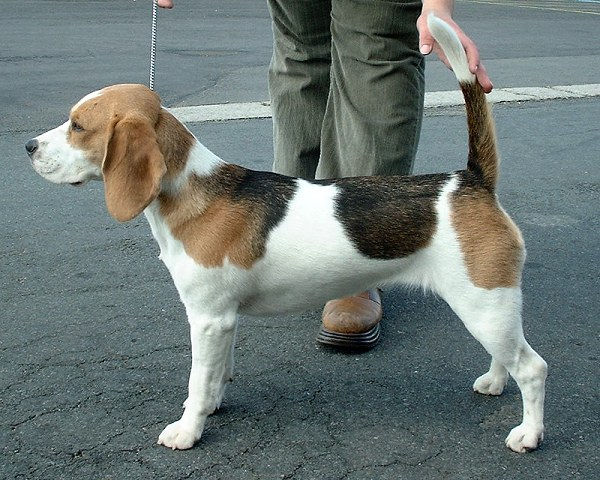
\includegraphics[width=0.9\linewidth]{Billeder/Jagthunde/stoevende/beagle.jpg} % Ikon af en drivende hund (f.eks. Beagle)

\end{columns}

\end{frame}

\begin{frame}{Schweisshunde (Specialister i eftersøgning)}

\vspace{1em}

\begin{columns}[c] % c = center vertically

\column{0.05\textwidth} % Venstre margin

\column{0.7\textwidth} % Midten: Bullets

\small

\raggedright

\begin{itemize}

\itemsep0.6em % Justér afstand mellem bullets

\item Hundens opgave er udelukkende at \textbf{eftersøge anskudt/trafikeret vildt} (Schweiss = blod (tysk)).
\item De arbejder i et spor, der kan være \textbf{flere timer gammelt}, primært i line (sporsele).
\item Enhver jæger har pligt til at \textbf{tilkalde en schweisshundefører}, hvis de anskyder klovbærende vildt.
\item Hundene har en \textbf{trænet lugtesans} og et roligt temperament.
\item \textbf{Racer}: Hannoversk Schweisshund, Bayersk Bjergschweisshund, og i Danmark ofte Ruhåret/Korthåret Hønsehund (som er godkendt til opgaven).

\end{itemize}

\column{0.25\textwidth} % Højre: Ikon

\centering

\vspace{0pt}

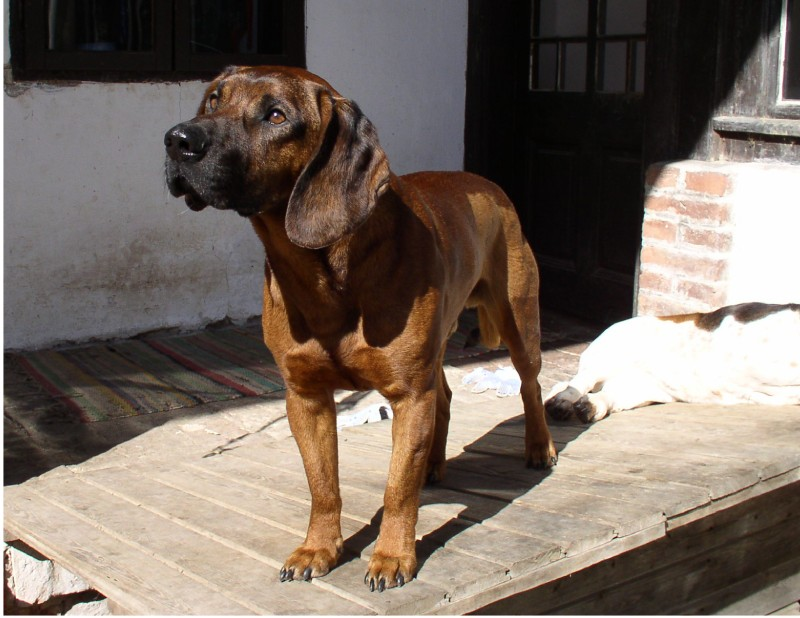
\includegraphics[width=0.9\linewidth]{Billeder/Jagthunde/schweisshunde/schweisshund.jpg} % Ikon af hund i sele/spor

\end{columns}

\end{frame}

\begin{frame}{Gravsøgende jagthunde}

\vspace{1em}

\begin{columns}[c] % c = center vertically

\column{0.05\textwidth} % Venstre margin

\column{0.7\textwidth} % Midten: Bullets

\small

\raggedright

\begin{itemize}

\itemsep0.6em % Justér afstand mellem bullets

\item Hundens opgave er at \textbf{lokalisere og drive vildtet ud af hulen} (gravjagt).
\item Anvendes primært til jagt på \textbf{ræv} i deres huler (grave).
\item Hundene skal have et \textbf{hårdt og modigt sind} og være fysisk rustede til trange miljøer.
\item Gravjagten er en \textbf{særlig jagtform} og er reguleret af Miljøstyrelsen.
\item \textbf{Racer}: Fox Terrier, Jack Russell Terrier, Tysk Jagtterrier, Gravhunde.

\end{itemize}

\column{0.25\textwidth} % Højre: Ikon

\centering

\vspace{0pt}

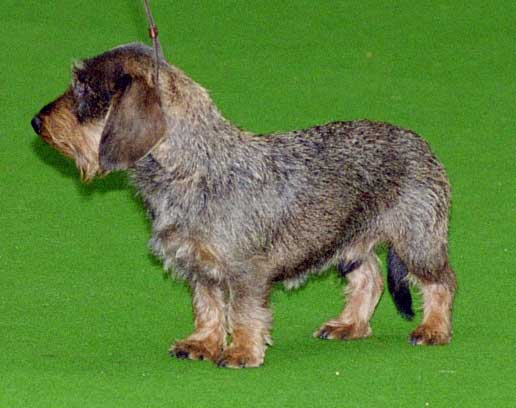
\includegraphics[width=0.9\linewidth]{Billeder/Jagthunde/gravsoegende/gravhund.jpg} % Ikon af gravsøgende hund/gravhund

\end{columns}

\end{frame}

\section{Håndtering af nedlagt vildt}

\begin{frame}
  \vspace{3em}
  \begin{center}
    {\LARGE \textbf{Håndtering af nedlagt vildt}
    }
    \\
    \vspace{1em}
    Hygiejnevejledningen
    \\
    \vspace{1em}
    Vejledning nr. 10099 af 20. december 2023, Kapitel 49
   \end{center}
\end{frame}



\begin{frame}{Affangning af anskudt vildt}
    \begin{itemize}
        \item Mål: Hurtig og smertefri aflivning af anskudt vildt
        \item Fuglevildt: Hårdt slag mod hoved/nakke (træstamme eller stok)
        \item Hare: Slag i nakken eller træk hoved/nakke nedad (hold i bagben)
        \item Rovvildt & større hjortevildt: Ekstra skud (undgå kniv – høj risiko)
        \item Ved brug af hund: Bevar overblik – vent med skud til sikkert
        \item Altid: Prioritér dyrevelfærd og jægersikkerhed
    \end{itemize}
\end{frame}
    

\begin{frame}{Opbrækning af vildt}
    \begin{itemize}
        \item \textbf{Formål}: Fjerne indvolde hurtigt for at undgå gæring, forurening og kødsurhed
        \item Gør det \textbf{straks} efter nedlæggelse (helst inden 30–60 min.)
        \item Grundtrin (klovbærende vildt):
          \begin{itemize}
            \item Læg dyret på ryggen (ben opad) – gerne på rent underlag
            \item Skær fra brystben til hale (åbn bughulen)
            \item Undgå at skære i tarmene/vommen – skær forsigtigt rundt om endetarm
            \item Udtag indvolde samlet (hjerte, lunger, lever, mave, tarme)
            \item Fjern spiserør og luftrør op mod halsen
            \item Tør bughulen ren med klud/papir (ingen vand!)
          \end{itemize}
        \item \textbf{Hygiejne}: Rene hænder/kniv, undgå jord/græs-kontakt
        \item Efter opbrækning: Afkøl hurtigt – hæng op i skygge/køligt sted
        \item https://www.facebook.com/reel/889956353611580
    \end{itemize}
\end{frame}




\begin{frame}{Forlægning af vildt}
    \begin{itemize}
        \item \textbf{Betydning}: Partering/udskæring af klovbærende vildt efter opbrækning
        \item Formål: Adskille kød fra knogler, flå skind af, forberede til modning/konsum
        \item Gøres typisk hjemme eller på jagtstedet efter indvolde er fjernet
        \item Grundtrin (eks. rådyr):
          \begin{itemize}
            \item Hæng dyret op (hoved opad) i køligt sted
            \item Flå skindet af (start ved baglår, træk ned mod hoved)
            \item Fjern hoved, ben og skanker i leddene
            \item Skær ud stykker: stege, culotte, fileter, bov, nakke m.m.
            \item Fjern sener, hinder og fedt efter behov
          \end{itemize}
        \item Hygiejne: Rene redskaber, arbejd køligt, undgå forurening
        \item Modning: Hæng kødet 4–10 dage (afhængig af temperatur (ikke over 7 grader), ca. 40 graddøgn)
    \end{itemize}
\end{frame}
\begin{frame}{Levering til vildthåndteringsvirksomhed – hovedregler}
    \begin{itemize}
        \item Hovedregel: Til vildthåndteringsvirksomhed (samme hygiejne som slagteri)
        \item Nedkøl hurtigt: ≤7 °C storvildt / ≤4 °C småvildt
        \item Luft om dyrene – ingen bunker
        \item Indlever alle dele + organer (undt. gevir/horn/stødtænder; mave/tarme for storvildt)
        \item Uddannet jæger OK → hoved/organer kan udelades (trikiner: altid med for visse arter)
        \item Unormalt: Alle dele med
    \end{itemize}
\end{frame}
\begin{frame}{Direkte afsætning af vildt – forbruger \& lokale butikker}
    \begin{itemize}
        \item Mindre mængder: Direkte til forbruger eller lokale butikker/restauranter
        \item Grænser: 500 småvildt + 15 storvildt pr. år
        \item Organer: Ikke påkrævet med
        \item Trikiner (fx vildsvin): Jæger sørger for undersøgelse
        \item Kontakt Fødevarestyrelsen for lab-info
    \end{itemize}
\end{frame}
\begin{frame}{Vildtdepoter – krav og indretning}
    \begin{itemize}
        \item Registrering: Direkte fra jægere → hos Fødevarestyrelsen
        \item Autorisation: Fra andre depoter
        \item Lager: Ikke nødvendigt inden 12 timer; ellers overdækket, rengørligt, luft om dyr
        \item Nedkøling: Naturlig OK i koldt vejr; aktiv ved sommer/lang tid
        \item Temperatur: ≤7 °C storvildt / ≤4 °C småvildt
        \item Undgå bunker for bedre afkøling
    \end{itemize}
\end{frame}
\begin{frame}{Primærproducenter vs. konsortier \& lodsejere}
    \begin{itemize}
        \item Enkelt jæger: Primærproducent → direkte salg til forbruger OK
        \item Konsortium som helhed / lodsejer: Ikke primærproducent → ingen direkte salg
        \item Løsning: Registrer som vildtdepot → levering til vildthåndteringsvirksomhed
        \item Direkte til forbruger: Via registreret detailudsalg
        \item Jagtparade: Salg til deltagere uden registrering (kun egen husholdning)
    \end{itemize}
\end{frame}
\begin{frame}{Uddannelse – krav til jægere ved markedsføring}
    \begin{itemize}
        \item Kendskab til: Vildtpatologi, håndtering af vildt \& kød
        \item Tilstrækkeligt: Én uddannet person pr. jagtselskab/konsortium
        \item Selskabet sikrer kravet opfyldes
        \item Kursus: Vildtsygdomme \& hygiejne (DJ m.fl.)
    \end{itemize}
\end{frame}
\begin{frame}{Vurdering af vildt (§49.6)}
    \begin{itemize}
        \item \textbf{Hovedregel}: Vildt/kød skal vurderes af \textbf{uddannet person} (se §49.5)
        \item \textbf{Undtagelse}: Ikke krav ved direkte levering til endelig forbruger eller lokale detailbutikker (restauranter, vildtbutikker, supermarkeder)
        \item \textbf{Vurderingens indhold}:
          \begin{itemize}
            \item Adfærd før nedlæggelse (observeret af uddannet person eller beskrevet af nedlæggeren)
            \item Krop og organer efter nedlæggelse (tegn på sygdom, forurening m.m.)
          \end{itemize}
        \item \textbf{Jægererklæring} (kun storvildt til vildthåndteringsvirksomhed):
          \begin{itemize}
            \item Udstedes af uddannet person
            \item Indeholder: Dato, tid, sted for nedlæggelse; navn, underskrift, evt. jagttegnsnummer
            \item Kan dække flere dyr (med identifikationsnumre)
            \item To standarder: Normal (alt OK) eller unormal (problemer konstateret)
          \end{itemize}
        \item \textbf{Uden uddannet person til stede}: Hoved + organer (undt. gevir/horn/stødtænder + mave/tarme) skal medfølge; stadig sporbarhed (jæger, sted, dato)
        \item Kilder: Hygiejneforordningen bilag III afsnit IV kap. I pkt. 3; kap. II pkt. 4a
    \end{itemize}
\end{frame}


\section{Eftersøgning}

\end{document}